\documentclass[12pt, letterpaper]{report} % Usa la clase report para documentos divididos en capítulos

%Paquete que da el formato al documento
\usepackage{pucv_inf_2024}
\usepackage{pdfpages}
\usepackage{tabularx}
\usepackage{caption}
\usepackage{lipsum}
\usepackage{graphicx}
\usepackage{biblatex}
\usepackage{pdflscape}
\usepackage{xltabular}
\usepackage{longtable}
\usepackage{booktabs}
\usepackage{placeins}
\usepackage{pgfplots}
\pgfplotsset{compat=1.18}
\usepackage{tikz}
\usetikzlibrary{arrows.meta, positioning, fit, backgrounds}
\usepackage{hyperref}
\hypersetup{
    colorlinks=true,
    linkcolor=black,
    citecolor=black,
    urlcolor=black
}

\renewcommand{\tablename}{Tabla}
\renewcommand{\figurename}{Figura}

% Código fuente en los anexos
\usepackage{listings}
\renewcommand{\lstlistingname}{Código}
\lstset{
    language=Python,
    basicstyle=\ttfamily\scriptsize,
    keywordstyle=\bfseries\color{blue!60!black},
    commentstyle=\itshape\color{gray},
    stringstyle=\color{teal!70!black},
    numbers=left, numberstyle=\tiny\color{gray}, numbersep=6pt,
    frame=tb, rulecolor=\color{gray!60},
    breaklines=true, breakatwhitespace=true, columns=fullflexible, keepspaces=true,
    showstringspaces=false, tabsize=4, xleftmargin=1.5em,
    literate={á}{{\'a}}1 {é}{{\'e}}1 {í}{{\'i}}1 {ó}{{\'o}}1 {ú}{{\'u}}1 {ñ}{{\~n}}1
             {Á}{{\'A}}1 {É}{{\'E}}1 {Í}{{\'I}}1 {Ó}{{\'O}}1 {Ú}{{\'U}}1 {Ñ}{{\~N}}1
             {ü}{{\"u}}1 {λ}{{$\lambda$}}1 {π}{{$\pi$}}1,
}

\addbibresource{referencias.bib}

% Glosario
\loadglsentries{glosario}
\makeglossaries

\begin{document}

%% TEX CON PORTADA DEL INFORME
% Portada para informes en asignaturas
%\title{Título del Informe\\[0.2cm] Segunda Línea del Título}
\author{Nombre y Apellido 1\\[0.2cm] Nombre y Apellido 2\\[0.2cm]...}
\date{Julio 2024}

\begin{titlepage}
  \addtocounter{page}{-1} 
  \makeatletter
  \thispagestyle{plain} % Usa el estilo 'plain' definido para la página de título
    
    \begin{picture}(0,0)
         \put(-75,-80){
\includegraphics[width=20cm]{Portadas/imagenes/encabezado.png}}
    \end{picture}

  \begin{flushright} % Alinea el contenido a la derecha
  \vspace*{\fill} % Centra verticalmente el contenido
    {\textcolor{titlecolor}{\LARGE\bfseries\MakeUppercase{
    \@title}}}
  \vspace*{\fill} % Centra verticalmente el contenido
  
    {\textcolor{titlecolor}{\Large\bfseries\textsc{
    \@author
    }}} \\[1cm]
    {\textcolor{titlecolor}{\bfseries\textsc{
    Nombre de la Asingatura\\[0.2cm] 
    \@date
    }}}

  \end{flushright}
\end{titlepage}

% Portada para informes de TFT a excepción del final de Proyecto
\title{Modelos Probabilísticos para la\\
        Detección de Amenazas Persistentes\\
        Avanzadas (APT)\\[9pt]}
\author{Francisca Antonia Abarca Pezo}
\newcommand{\prof}{Sebastián Berrios}
\newcommand{\corprof}{Pamela Hermosilla}
\date{Noviembre 2026}


\begin{titlepage}
  \makeatletter
  \thispagestyle{empty} % Usa el estilo 'plain' definido para la página de título
    %\begin{center}
    
    \begin{picture}(0,0)
         \put(-75,-80){
\includegraphics[width=20cm]{Portadas/imagenes/encabezado.png}}
    \end{picture}
    %\end{center}

  
  \begin{flushright} % Alinea el contenido a la derecha
  \vspace*{\fill} % Centra verticalmente el contenido
    {\textcolor{titlecolor}{\LARGE\bfseries\MakeUppercase{
    \@title}}}
  
    {\textcolor{titlecolor}{\Large\bfseries\textsc{\@author}}} \\[4cm]
    
    {\textcolor{titlecolor}{\large\bfseries\textsc{Profesor Guía: \prof}}} \\[10pt]
    {\textcolor{titlecolor}{\large\bfseries\textsc{Profesora Correferente: \corprof}}} \\[2cm]

    %\vspace*{\fill} % Centra verticalmente el contenido
    {\textcolor{titlecolor}{\bfseries\textsc{Informe Final de Seminario de Título\\[0.2cm]Ingeniería Civil Informática\\[0.2cm]\@date
    }}}

  \end{flushright}  
\end{titlepage}

% Portada informe final de proyecto 
%
\title{Título del Tema del TFT}
\author{Nombre Estudiante 1\\[10pt]Nombre Estudiante 2}
\renewcommand{\prof}{Nombre Profesor}
\renewcommand{\corprof}{Nombre Profesor Correferente}
\date{Julio 2024}


\begin{titlepage}
  \makeatletter
  \thispagestyle{empty} % Usa el estilo 'plain' definido para la página de título
    %\begin{center}
    
    \begin{picture}(0,0)
         \put(-75,-80){
\includegraphics[width=20cm]{Portadas/imagenes/encabezado.png}}
    \end{picture}
    %\end{center}

  
  \begin{flushright} % Alinea el contenido a la derecha
  \vspace*{\fill} % Centra verticalmente el contenido
    {\textcolor{titlecolor}{\LARGE\bfseries\MakeUppercase{
    \@title}}}
  
    {\textcolor{titlecolor}{\Large\bfseries\textsc{\@author}}} \\[3.5cm]
    
    {\textcolor{titlecolor}{\large\bfseries\textsc{Profesor Guía: \prof}}} \\[10pt]
    {\textcolor{titlecolor}{\large\bfseries\textsc{Profesor Correferente: \corprof}}} \\[2cm]

    %\vspace*{\fill} % Centra verticalmente el contenido
    {\textcolor{titlecolor}{\bfseries\textsc{Informe final de Proyecto de Título\\[0.2cm]Para Optar al Título Profesional de\\[0.2cm]Nombre del Título Profesional\\[0.2cm]\@date
    }}}

  \end{flushright}  
\end{titlepage}

%% DEDICATORIA (incluir solo en TFT y TFG, sino comentar)
%\chapter*{} 
\vfill % Empuja el contenido siguiente al fondo de la página
\hfill % Alinea el contenido siguiente a la derecha
\begin{minipage}{\textwidth}
\raggedleft % Asegura que el texto dentro de minipage esté alineado a la derecha
\it{Dedicatoria (se incluye solo en TFT o TFG).\\
Una dedicatoria es una breve expresión de gratitud\\
o reconocimiento, generalmente personal y emotiva,\\ 
donde el autor dedica su trabajo a una o\\
varias personas significativas en su vida.}
\end{minipage}
\addtocounter{page}{-1} 

%% RESUMEN/ABSTRACT DEL INFORME
\chapter*{Resumen}
\addcontentsline{toc}{chapter}{Resumen/Abstract\vspace{-0.5cm}}

Las Amenazas Persistentes Avanzadas corresponden a campañas de ataque dirigidas y sigilosas que se desarrollan en múltiples etapas a lo largo de meses, lo que les permite evadir los mecanismos de detección tradicionales. Estos mecanismos evalúan eventos de forma aislada y no la secuencia temporal completa que caracteriza a este tipo de campañas, situación que se ve agravada por el severo desbalance entre tráfico legítimo y malicioso presente en los escenarios reales de operación.

Este trabajo propone la implementación y validación de un modelo basado en Cadenas Ocultas de Markov para la detección de este tipo de amenazas a partir de tráfico de red, representando las etapas del ataque como estados no observables que se infieren desde la evidencia disponible. La investigación se enmarca en la metodología de Design Science Research y se sustenta en una revisión sistemática de la literatura, que fundamenta tanto la selección del enfoque probabilístico como el diseño del modelo y de los conjuntos de datos empleados para su evaluación.

La revisión sistemática, ejecutada sobre Scopus, Web of Science e IEEE Xplore, conformó un corpus de 77 estudios primarios y permitió identificar cuatro brechas: la dependencia de alertas previamente correlacionadas, la escasa aplicación de estos modelos directamente sobre tráfico de red, la falta de un conjunto de datos de referencia consolidado y el predominio de métricas globales que ocultan el desempeño sobre la clase minoritaria. A partir de ellas se diseñó un modelo cuyos estados se anclan a las etapas etiquetadas de los conjuntos DAPT2020 y Unraveled, que trata el desbalance sin alterar la estructura temporal de las secuencias y que se evalúa mediante métricas por etapa y de detección temprana, en comparación con Random Forest y XGBoost bajo las mismas condiciones experimentales. Un prototipo implementado en Python y evaluado de forma preliminar sobre ambos conjuntos muestra que la estimación supervisada conserva la correspondencia entre estados y etapas que el entrenamiento no supervisado pierde, mientras que con la configuración actual los modelos de referencia superan al modelo propuesto en la clasificación por ventana y en la detección a igual tasa de falsas alarmas. Estos resultados orientan los ajustes del diseño, como el análisis de la campaña a nivel de red y la selección del tamaño de ventana y de la discretización.

{\bf Palabras clave:} amenazas persistentes avanzadas, cadenas ocultas de Markov, detección temprana, detección de intrusiones, revisión sistemática de literatura, desbalance de clases


\clearpage
\chapter*{Abstract}
Advanced Persistent Threats are targeted, stealthy attack campaigns that unfold across multiple stages over several months, allowing them to evade traditional detection mechanisms. These mechanisms assess events in isolation rather than the full temporal sequence that characterises such campaigns, a limitation compounded by the severe imbalance between legitimate and malicious traffic found in real operating environments.

This work proposes the implementation and validation of a Hidden Markov Model for detecting this type of threat from network traffic, representing attack stages as unobservable states inferred from the available evidence. The research follows the Design Science Research methodology and is grounded in a systematic literature review, which supports the selection of the probabilistic approach as well as the design of the model and the datasets used for its evaluation.

The systematic review, conducted on Scopus, Web of Science and IEEE Xplore, yielded a corpus of 77 primary studies and revealed four gaps: reliance on previously correlated alerts, the limited application of these models directly to network traffic, the lack of a consolidated benchmark dataset, and the prevalence of global metrics that conceal performance on the minority class. Building on these gaps, the proposed model anchors its states to the labelled stages of the DAPT2020 and Unraveled datasets, handles class imbalance without altering the temporal structure of the sequences, and is evaluated with per-stage and early-detection metrics against Random Forest and XGBoost under the same experimental conditions. A Python prototype, evaluated in a preliminary way on both datasets, shows that supervised estimation preserves the correspondence between states and stages that unsupervised training loses, whereas with the current configuration the baseline models outperform the proposed model in window-level classification and in detection at equal false alarm rates. These results guide the design adjustments, such as a network-level analysis of the campaign and the selection of the window size and the discretization.

{\bf Keywords:} advanced persistent threats, hidden Markov models, early detection, intrusion detection, systematic literature review, class imbalance


%% INDICE, LISTAS de FIGURAS/TABLAS/ALGORITMOS, GLOSARIO, ETC.
%% COMENTAR EN CASO DE NO QUERER INCLUIR ALGUNA DE ESTAS LISTAS/INDICES
\newpage\addcontentsline{toc}{chapter}{Índice General\vspace{-0.5cm}}
\tableofcontents % Este comando genera el índice

\newpage\addcontentsline{toc}{chapter}{Lista de Figuras\vspace{-0.5cm}}
\listoffigures % Índice de figuras

\newpage\addcontentsline{toc}{chapter}{Lista de Tablas\vspace{-0.5cm}}
\listoftables  % Índice de tablas

%\newpage\addcontentsline{toc}{chapter}{Lista de Algoritmos\vspace{-0.5cm}}
%\listofalgorithms 

% Lista de Símbolos
%%% LISTA DE SIMBOLOS

\nomenclature{$\sin$}{Función seno}
\nomenclature{$\cos$}{Función coseno}
\nomenclature{$\pi$}{Número pi}
\nomenclature{$L$}{Longitud del intervalo asociado a la serie de Fourier}
%\newpage\addcontentsline{toc}{chapter}{Lista de Símbolos\vspace{-0.5cm}}
%\printnomenclature

%% GLOSARIO

\newacronym{apa}{APA}{American Psychological Association}
\newacronym{ats}{ATS}{Advanced Terrestrial Simulator}\glsaddall
%\addcontentsline{toc}{chapter}{Glosario}
%\printglossary[type=\acronymtype]

\newpage
\pagenumbering{arabic} % Cambia a numeración arábiga para el resto del documento

% CONTENIDO PRINCIPAL DEL DOCUMENTO
\chapter{Introducción}

La creciente digitalización de las operaciones institucionales ha ampliado de forma sostenida la superficie de exposición de las organizaciones frente a ataques informáticos. Dentro de este panorama, las Amenazas Persistentes Avanzadas (APT) ocupan un lugar particular: se trata de campañas dirigidas, ejecutadas por adversarios con recursos y objetivos definidos, que se despliegan de manera sigilosa a lo largo de meses y en múltiples etapas sucesivas \parencite{hutchins2011killchain}. Su impacto se extiende más allá del incidente puntual y compromete de forma prolongada la confidencialidad de la información de la organización afectada.

La dificultad para enfrentarlas radica en que los mecanismos de detección predominantes fueron diseñados para identificar eventos aislados y no secuencias de acciones distribuidas en el tiempo, razón por la cual las APT logran evadirlos con frecuencia \parencite{alshamrani2019survey}. Esta limitación ha motivado el interés por enfoques capaces de modelar la progresión de un ataque como un proceso, incorporando la incertidumbre inherente al comportamiento del adversario. Entre ellos, los modelos probabilísticos ofrecen un marco formal para estimar en qué etapa de una campaña se encuentra un atacante a partir de la evidencia observable en la red.

El presente proyecto aborda esta problemática mediante la implementación y validación de un modelo basado en Cadenas Ocultas de Markov (HMM) para la detección de APT, evaluado empíricamente sobre dos conjuntos de datos complementarios: DAPT2020 \parencite{myneni2020dapt2020}, que permite la comparación con los enfoques reportados en la literatura, y Unraveled \parencite{myneni2023unraveled}, que reproduce condiciones de operación más realistas mediante la emulación de seis semanas de actividad organizacional. Ambos fueron seleccionados mediante criterios explícitos derivados de los requerimientos del modelo: campañas APT multietapa, etiquetas de etapa por registro, tráfico de red a nivel de flujo y actividad benigna continua. La investigación se enmarca en la metodología de Design Science Research \parencite{peffers2007dsrm}, orientada a la construcción de artefactos que resuelven problemas concretos, y se apoya en una revisión sistemática de la literatura para fundamentar las decisiones de diseño del modelo propuesto.

Este documento corresponde al Informe Final de Seminario de Título y se organiza de la siguiente manera. El Capítulo~2 describe el problema abordado y su relevancia. El Capítulo~3 define el objetivo general y los objetivos específicos del proyecto. El Capítulo~4 presenta el marco teórico con los conceptos y técnicas necesarios para comprender la propuesta. El Capítulo~5 detalla la metodología de investigación adoptada y el procedimiento seguido en la revisión sistemática de la literatura. El Capítulo~6 expone el estado del arte resultante de dicha revisión. El Capítulo~7 presenta el plan de trabajo y su cronograma para ambos semestres. El Capítulo~8 describe la propuesta de solución y su diseño experimental. El Capítulo~9 presenta una primera implementación de la propuesta y sus resultados preliminares sobre ambos conjuntos de datos. El Capítulo~10 recoge las conclusiones de esta etapa y el Capítulo~11 declara el uso de herramientas de inteligencia artificial en la elaboración del documento.
\chapter{Descripción del Problema}

Las Amenazas Persistentes Avanzadas (APT) constituyen una de las formas de ataque más difíciles de enfrentar en la ciberseguridad actual. A diferencia de un ataque puntual, una APT corresponde a una campaña dirigida y sigilosa que puede extenderse durante meses y que se desarrolla en múltiples etapas sucesivas, desde el reconocimiento inicial del objetivo hasta la exfiltración de información \parencite{hutchins2011killchain}. Esta naturaleza prolongada y por etapas es precisamente lo que les permite operar sin ser detectadas: cada acción individual del atacante, observada de forma aislada, resulta indistinguible de la actividad legítima de la red.

El problema radica en que los mecanismos de detección tradicionales no están diseñados para capturar este comportamiento. Las herramientas basadas en firmas estáticas, así como buena parte de los sistemas de detección de intrusiones convencionales, evalúan eventos de manera aislada y no la secuencia temporal completa que caracteriza a una campaña de este tipo, por lo que las APT logran evadirlos con frecuencia \parencite{alshamrani2019survey}. A esta limitación se suma una segunda dificultad, esta vez en el plano de los datos disponibles para investigación: los conjuntos de datos de intrusiones genéricos presentan una diferencia demasiado evidente entre el tráfico normal y el anómalo, lo que no representa la sofisticación real de un atacante APT, y su distribución de clases no refleja las condiciones reales de operación \parencite{myneni2020dapt2020}. En escenarios reales, la actividad maliciosa constituye una fracción mínima del tráfico total, un desbalance severo que dificulta tanto el entrenamiento como la evaluación de modelos de detección.

Es necesario distinguir entre el problema general y la brecha específica que aborda esta investigación. La detección de APT ha sido ampliamente estudiada, y existen enfoques que incorporan la dimensión temporal del ataque mediante modelos de progresión por etapas. Por tanto, la brecha está en las condiciones bajo las cuales estas propuestas han sido validadas. Los trabajos existentes tienden a evaluarse sobre conjuntos de datos con distribuciones de clase artificialmente equilibradas o con una separación demasiado evidente entre tráfico legítimo y malicioso, escenarios que no reproducen las condiciones reales de operación. En consecuencia, permanece abierta la pregunta de si los enfoques probabilísticos secuenciales mantienen su desempeño cuando la actividad maliciosa constituye una fracción mínima del tráfico total, condición que caracteriza a los entornos reales y que este trabajo aborda de manera explícita.

Las consecuencias de esta brecha son concretas. Una campaña que permanece activa durante meses sin ser detectada implica pérdida sostenida de información confidencial, un tiempo de respuesta que se mide en semanas o meses en lugar de horas, y la imposibilidad de intervenir en las etapas tempranas del ataque, cuando el daño aún es limitado. Existe, por tanto, la necesidad de enfoques de detección capaces de razonar sobre la progresión temporal de un ataque y de hacerlo bajo las condiciones de desbalance de datos que caracterizan a los escenarios reales. Esta situación se evidencia en trabajos recientes: al evaluar modelos de detección de anomalías ampliamente utilizados sobre un escenario que emula seis semanas de actividad organizacional real, la actividad correspondiente a la campaña APT resulta prácticamente indetectable \parencite{myneni2023unraveled}.
\chapter{Definición de objetivos}

\section{Objetivo General}
\vspace{-0.17cm}
Desarrollar un modelo probabilístico basado en Cadenas Ocultas de Markov que permita detectar Amenazas Persistentes Avanzadas mediante la identificación temprana de su progresión por etapas.
\vspace{-0.35cm}

\section{Objetivos Específicos}
\vspace{-0.1cm}
Los objetivos específicos se organizan en tres dimensiones metodológicas: \textbf{Estudio}, \textbf{Desarrollo} y \textbf{Validación}, las cuales cubren el ciclo completo del proyecto desde la revisión del conocimiento existente hasta la evaluación empírica de la propuesta.
\vspace{-0.45cm}

\begin{center}
    \small
    \renewcommand{\arraystretch}{1.3}

    % --- TABLA 1: ESTUDIO ---
    \begin{tabularx}{\textwidth}{|c|X|}
    \hline
    \multicolumn{2}{|l|}{\textbf{Dimensión: Estudio}} \\ \hline
    \textbf{OE1} & Realizar una revisión sistemática de literatura (SLR), conforme a las directrices de Kitchenham y Charters \parencite{kitchenham2007guidelines} y reportada según la declaración PRISMA \parencite{page2021prisma}, para identificar, analizar y sintetizar las principales contribuciones científicas sobre modelos probabilísticos aplicados a la detección de Amenazas Persistentes Avanzadas, con énfasis en enfoques basados en Modelos Ocultos de Markov, identificando las limitaciones de los enfoques existentes y las brechas que justifican la propuesta. \\ \hline
    \textbf{OE2} & Formular un marco formal que caracterice los estados ocultos y las variables observables del proceso de una APT, en base a las etapas de ataque y las características del tráfico definidas en los conjuntos de datos DAPT2020 y Unraveled, identificando los criterios que debe satisfacer el modelo para representar la progresión del ataque. \\ \hline
    \end{tabularx}
    \captionof{table}{Objetivos específicos correspondientes a la dimensión de Estudio.}
    \label{tab:obj_estudio}
    
    \vspace{0cm}

    % --- TABLA 2: DESARROLLO ---
    \begin{tabularx}{\textwidth}{|c|X|}
    \hline
    \multicolumn{2}{|l|}{\textbf{Dimensión: Desarrollo}} \\ \hline
    \textbf{OE3} & Diseñar la arquitectura del modelo HMM para la detección de APT, especificando sus componentes (estados ocultos, variables observables, matrices de transición y emisión), los algoritmos de entrenamiento e inferencia a utilizar (estimación supervisada con refinamiento mediante Baum-Welch, inferencia filtrada y Viterbi), los mecanismos que aseguran la correspondencia entre los estados aprendidos y las etapas de ataque, y el flujo de datos desde el preprocesamiento de los conjuntos de datos hasta la entrada del modelo. \\ \hline
    \textbf{OE4} & Implementar un prototipo funcional del modelo HMM que procese el tráfico de red de los conjuntos de datos seleccionados, infiera la secuencia más probable de etapas de una APT en curso y reporte dicha progresión junto con las probabilidades asociadas a cada etapa. \\ \hline
    \end{tabularx}
    \captionof{table}{Objetivos específicos correspondientes a la dimensión de Desarrollo.}
    \label{tab:obj_desarrollo}
    
    \vspace{0cm}

    % --- TABLA 3: VALIDACIÓN ---
    \begin{tabularx}{\textwidth}{|c|X|}
    \hline
    \multicolumn{2}{|l|}{\textbf{Dimensión: Validación}} \\ \hline
    \textbf{OE5} & Evaluar el desempeño del modelo HMM mediante experimentos controlados sobre los conjuntos de datos DAPT2020 y Unraveled, considerando métricas de precisión, exhaustividad y F1-score por etapa de ataque, métricas de detección temprana (tiempo hasta la detección y detección previa a la exfiltración, en relación con la tasa de falsas alarmas) y el efecto del desbalance de clases, comparándolo con modelos de referencia (Random Forest y XGBoost) implementados bajo las mismas condiciones experimentales. \\ \hline
    \end{tabularx}
    \captionof{table}{Objetivo específico correspondiente a la dimensión de Validación.}
    \label{tab:obj_validacion}

\end{center}
\chapter{Marco Teórico}
En este capítulo se presentan los fundamentos conceptuales y matemáticos que sustentan el desarrollo de la investigación. Se formalizan las características operacionales de las Amenazas Persistentes Avanzadas, los fundamentos teóricos de los Modelos Ocultos de Markov (HMM), los algoritmos de entrenamiento e inferencia y sus limitaciones, las técnicas para abordar el desbalance severo de clases y los modelos de referencia con que se contrastará la propuesta.

\section{Amenazas Persistentes Avanzadas (APT)}
Una Amenaza Persistente Avanzada (APT) es una campaña de intrusión dirigida, sigilosa y estructurada en múltiples fases sucesivas ejecutada por actores con capacidades técnicas avanzadas \parencite{hutchins2011killchain}. A diferencia del malware convencional, una APT no persigue la disrupción inmediata, sino la permanencia prolongada dentro de la infraestructura para exfiltrar activos estratégicos.

Formalmente, el ciclo de vida de una APT se modela a través de la \textit{Cyber Kill Chain} o la matriz \textit{MITRE ATT\&CK}, transitando por una secuencia finita y ordenada de etapas:
\begin{equation}
\mathcal{E} = \{e_{\text{recon}}, e_{\text{foothold}}, e_{\text{lateral}}, e_{\text{exfil}}\}
\end{equation}
donde cada fase presenta tácticas y patrones de tráfico de red específicos. Dado que las acciones individuales imitan el tráfico benigno, su identificación requiere modelar la dependencia temporal entre eventos secuenciales.

\section{Modelos Ocultos de Markov (HMM)}
Un Modelo Oculto de Markov es un modelo estadístico generativo en el cual el sistema modelado es un proceso estocástico de Markov con estados no directamente observables (ocultos), pero inferibles a través de un conjunto de observaciones estocásticas generadas por dichos estados \parencite{rabiner1989}.

Formalmente, un HMM se define mediante la 5-tupla $\lambda = (S, V, A, B, \pi)$:
\begin{enumerate}
    \item \textbf{Conjunto de estados ocultos:} $S = \{s_1, s_2, \dots, s_N\}$, donde $N$ representa el número de estados en el modelo (correspondientes a las etapas de la APT y el estado benigno). El estado en el instante temporal $t$ se denota como $q_t \in S$.
    \item \textbf{Conjunto de observaciones discretas:} $V = \{v_1, v_2, \dots, v_M\}$, donde $M$ representa la cardinalidad del espacio de observaciones observables derivadas del tráfico de red. La observación en el instante $t$ se denota como $O_t \in V$.
    \item \textbf{Matriz de transición de estados ($A$):} Define la probabilidad de transitar de un estado $s_i$ a un estado $s_j$:
    \begin{equation}
    A = [a_{ij}], \quad a_{ij} = P(q_{t+1} = s_j \mid q_t = s_i), \quad 1 \le i, j \le N
    \end{equation}
    sujeta a las restricciones estocásticas $a_{ij} \ge 0$ y $\sum_{j=1}^N a_{ij} = 1$.
    \item \textbf{Matriz de probabilidades de emisión ($B$):} Define la probabilidad de generar una observación observable $v_k$ dado que el sistema se encuentra en el estado oculto $s_j$:
    \begin{equation}
    B = [b_j(k)], \quad b_j(k) = P(O_t = v_k \mid q_t = s_j), \quad 1 \le j \le N, \, 1 \le k \le M
    \end{equation}
    con $b_j(k) \ge 0$ y $\sum_{k=1}^M b_j(k) = 1$.
    \item \textbf{Distribución de estados iniciales ($\pi$):} Vector de probabilidades de inicio del proceso:
    \begin{equation}
    \pi = [\pi_i], \quad \pi_i = P(q_1 = s_i), \quad 1 \le i \le N, \quad \sum_{i=1}^N \pi_i = 1
    \end{equation}
\end{enumerate}

\subsection{Algoritmo de Inferencia: Decodificación de Viterbi}
Dado un modelo calibrado $\lambda = (A, B, \pi)$ y una secuencia de tráfico observada $O = (O_1, O_2, \dots, O_T)$, el problema de inferencia consiste en encontrar la secuencia de estados ocultos más probable $Q^* = (q_1^*, q_2^*, \dots, q_T^*)$ que optimiza $P(Q \mid O, \lambda)$. 

El algoritmo de Viterbi resuelve esta optimización mediante programación dinámica definiendo la variable de mejor puntaje $\delta_t(i)$:
\begin{equation}
\delta_t(i) = \max_{q_1, q_2, \dots, q_{t-1}} P(q_1 q_2 \dots q_t = s_i, O_1 O_2 \dots O_t \mid \lambda)
\end{equation}
cuya recursión para $1 \le t \le T-1$ y $1 \le j \le N$ corresponde a:
\begin{equation}
\delta_{t+1}(j) = \left[ \max_{1 \le i \le N} \delta_t(i) a_{ij} \right] \cdot b_j(O_{t+1})
\end{equation}
almacenando el puntero hacia atrás $\psi_{t+1}(j) = \arg\max_{1 \le i \le N} [\delta_t(i) a_{ij}]$ para reconstruir la trayectoria causal del atacante al tiempo $T$.

\subsection{Algoritmo de Entrenamiento: Baum-Welch (Expectation-Maximization)}
La estimación de los parámetros $\lambda = (A, B, \pi)$ a partir de secuencias de tráfico no etiquetadas o semi-supervisadas se lleva a cabo mediante el algoritmo de Baum-Welch, el cual maximiza iterativamente la función de verosimilitud $P(O \mid \lambda)$ mediante las probabilidades forward ($\alpha_t$) y backward ($\beta_t$):
\begin{align}
\alpha_t(i) &= P(O_1 O_2 \dots O_t, q_t = s_i \mid \lambda) \\
\beta_t(i) &= P(O_{t+1} O_{t+2} \dots O_T \mid q_t = s_i, \lambda)
\end{align}
Las probabilidades marginales a posteriori $\gamma_t(i)$ y $\xi_t(i, j)$ permiten recalcular de forma analítica las matrices de transición y emisión en cada iteración del paso $M$.

Al tratarse de un procedimiento de máxima verosimilitud con datos incompletos, Baum-Welch presenta dos propiedades que condicionan su uso en este trabajo. En primer lugar, converge a un máximo local de la verosimilitud, por lo que el modelo obtenido depende de la estimación inicial de $\lambda$ \parencite{rabiner1989}. En segundo lugar, la verosimilitud $P(O \mid \lambda)$ es invariante ante cualquier permutación de los índices de los estados aplicada de forma consistente sobre $A$, $B$ y $\pi$. En consecuencia, un HMM entrenado sin supervisión aprende estados que explican estadísticamente las observaciones, pero nada asegura que un estado determinado corresponda a una etapa concreta del ataque, como el movimiento lateral: la interpretación de los estados debe imponerse en el entrenamiento o verificarse después de él. Una propiedad útil para lo primero es que todo parámetro inicializado en cero permanece en cero durante la reestimación \parencite{rabiner1989}, lo que permite fijar la estructura de transiciones admitidas.

\subsection{Estimación supervisada de los parámetros}
Cuando las secuencias de entrenamiento cuentan con la secuencia de estados verdadera, como ocurre en conjuntos de datos etiquetados por etapa de ataque, los parámetros de máxima verosimilitud se obtienen en forma cerrada por conteo de frecuencias:
\begin{equation}
\hat{a}_{ij} = \frac{n_{ij} + \alpha}{\sum_{l=1}^{N} n_{il} + N\alpha}, \qquad
\hat{b}_j(k) = \frac{m_j(k) + \alpha}{\sum_{l=1}^{M} m_j(l) + M\alpha}, \qquad
\hat{\pi}_i = \frac{c_i + \alpha}{\sum_{l=1}^{N} c_l + N\alpha}
\end{equation}
donde $n_{ij}$ es el número de transiciones observadas de $s_i$ a $s_j$, $m_j(k)$ el número de veces que se emite el símbolo $v_k$ estando en $s_j$, $c_i$ el número de secuencias que comienzan en $s_i$, y $\alpha > 0$ un término de suavizado de Laplace que evita asignar probabilidad nula a transiciones o símbolos no observados en el entrenamiento. A diferencia de Baum-Welch, esta estimación vincula cada estado con su etiqueta por construcción.

\subsection{Inferencia en línea: probabilidad filtrada}
El algoritmo de Viterbi decodifica la secuencia completa $O_1, \dots, O_T$, de modo que la etapa asignada al instante $t$ puede depender de observaciones posteriores a $t$. Para un detector que debe emitir alertas a medida que llega el tráfico, la cantidad pertinente es la probabilidad filtrada, que solo utiliza la evidencia disponible hasta $t$ y se obtiene de la variable \textit{forward}:
\begin{equation}
P(q_t = s_i \mid O_1, \dots, O_t, \lambda) = \frac{\alpha_t(i)}{\sum_{j=1}^{N} \alpha_t(j)}
\end{equation}
Esta distribución se actualiza de forma recursiva con cada nueva observación y permite reportar, en cada instante, la etapa más probable junto con su nivel de confianza.

\section{Tratamiento del Desbalance Severo de Clases}
En entornos reales de detección de intrusiones, la actividad de un atacante APT representa una fracción marginal ($< 0.1\%$) del volumen total de registros de red \parencite{myneni2020dapt2020}. Esta desproporción introduce sesgos críticos en clasificadores discriminativos tradicionales, los cuales tienden a ignorar la clase minoritaria.

Un HMM modela la distribución conjunta $P(O, Q)$ en lugar de la frontera condicional $P(Q \mid O)$. Bajo estimación supervisada, cada fila de $B$ se estima únicamente con las observaciones de su propio estado y se normaliza por separado, de modo que el volumen de tráfico benigno no altera directamente el perfil de emisión de las etapas minoritarias. El desbalance se manifiesta, en cambio, en la escasez de transiciones observadas hacia y entre las etapas de ataque, que el suavizado de Laplace y la calibración del umbral de decisión sobre la probabilidad filtrada permiten compensar.

La técnica de remuestreo más difundida es SMOTE (\textit{Synthetic Minority Over-sampling Technique}) \parencite{chawla2002smote}, que genera nuevas instancias de la clase minoritaria por interpolación lineal entre una muestra y uno de sus $k$ vecinos más cercanos de la misma clase:
\begin{equation}
x_{\text{nuevo}} = x_i + \delta \cdot (x_{zi} - x_i), \quad \delta \in [0, 1]
\end{equation}
SMOTE trata cada instancia como independiente de las demás. Este supuesto es adecuado para clasificadores que evalúan cada ventana por separado, pero entra en conflicto con un modelo secuencial por tres razones:
\begin{enumerate}
    \item \textbf{Las instancias sintéticas no tienen posición temporal.} Una ventana generada por interpolación carece de antecesora y sucesora reales, por lo que no aporta información válida a la matriz de transición $A$. Si se inserta en una secuencia, introduce transiciones que no ocurrieron y altera la duración aparente de las etapas.
    \item \textbf{La interpolación no está definida sobre símbolos discretos.} El HMM opera sobre un alfabeto $V$ obtenido por discretización; interpolar entre dos símbolos produce valores intermedios sin significado o símbolos que no corresponden a ningún patrón de tráfico observado.
    \item \textbf{Riesgo de filtración de información.} Si el sobremuestreo se aplica antes de particionar los datos, instancias sintéticas derivadas de muestras de evaluación pueden quedar en el entrenamiento, lo que sobreestima el desempeño.
\end{enumerate}
Por estas razones, en este trabajo SMOTE no se aplica sobre las secuencias que alimentan al HMM. El tratamiento del desbalance para el modelo secuencial y el uso de SMOTE en el modelo de referencia se detallan en el Capítulo~\ref{cap:propuesta}.

\section{Modelos de referencia basados en ensambles de árboles}
Para determinar si el modelado secuencial aporta una mejora real, el desempeño del HMM se contrasta con clasificadores discriminativos que evalúan cada ventana de tráfico de forma independiente. Se consideran dos ensambles de árboles de decisión de uso extendido en la detección de intrusiones:
\begin{itemize}
    \item \textbf{Random Forest} \parencite{breiman2001random}: combina un conjunto de árboles entrenados sobre muestras \textit{bootstrap} de los datos y sobre subconjuntos aleatorios de atributos en cada división, y asigna la clase por votación mayoritaria. La aleatorización reduce la varianza respecto de un árbol individual.
    \item \textbf{XGBoost} \parencite{chen2016xgboost}: construye árboles de forma secuencial, de modo que cada uno corrige el error residual de los anteriores mediante \textit{gradient boosting} con regularización explícita de la complejidad del modelo.
\end{itemize}
Ambos admiten ponderación de clases y pueden combinarse con SMOTE, ya que tratan las ventanas como instancias independientes. Esa misma independencia les impide representar la progresión entre etapas, lo que los convierte en la línea base adecuada para aislar el aporte de la dimensión temporal del HMM.
\chapter{Metodología}

Dado que el resultado esperado de este trabajo es un artefacto, un modelo basado en Cadenas Ocultas de Markov, implementado y validado empíricamente sobre datos reales, la investigación adopta como metodología el Design Science Research (DSR) propuesto por Peffers et al. \parencite{peffers2007dsrm}, orientado a disciplinas centradas en la creación de artefactos que resuelven problemas concretos. Esta metodología estructura el proceso de investigación en seis fases, las cuales se corresponden con las dimensiones metodológicas definidas para los objetivos específicos de este proyecto, según se detalla en la Tabla~\ref{tab:dsr}.

\begin{table}[h!]
\centering
\small
\caption{Correspondencia entre las fases del ciclo DSR y las dimensiones del proyecto.}
\label{tab:dsr}
\begin{tabular}{p{7.2cm} p{3cm} p{4.4cm}}
\hline
\textbf{Fase DSR} & \textbf{Dimensión} & \textbf{Objetivos asociados} \\
\hline
1. Identificación del problema y motivación & Estudio & OE1 \\
2. Definición de los objetivos de la solución & Estudio & OE1, OE2 \\
3. Diseño y desarrollo & Desarrollo & OE3, OE4 \\
4. Demostración & Validación & OE5 \\
5. Evaluación & Validación & OE5 \\
6. Comunicación & --- & Informe y defensa \\
\hline
\end{tabular}
\end{table}

Las dos primeras fases del ciclo requieren caracterizar el estado actual del conocimiento sobre el problema abordado. Para ello se emplea como método una Revisión Sistemática de la Literatura (SLR), conducida conforme a las directrices de Kitchenham y Charters \parencite{kitchenham2007guidelines}, que estructuran este tipo de estudio en tres fases, planificación, ejecución y reporte, con el fin de asegurar un proceso reproducible y auditable. La documentación del proceso de identificación, cribado y selección de estudios se realiza siguiendo la declaración PRISMA 2020 \parencite{page2021prisma}, empleada aquí como guía de reporte y no como metodología de investigación.

La Figura~\ref{fig:dsr} presenta el esquema integrado de la metodología, indicando para cada fase del ciclo sus entradas, actividades y salidas. Como se observa, la Revisión Sistemática de la Literatura constituye la actividad central de las dos primeras fases, y sus salidas (el estado del arte y las brechas identificadas) corresponden a las entradas directas de la fase de diseño y desarrollo.

\begin{figure}[h!]
\centering
\resizebox{\textwidth}{!}{%
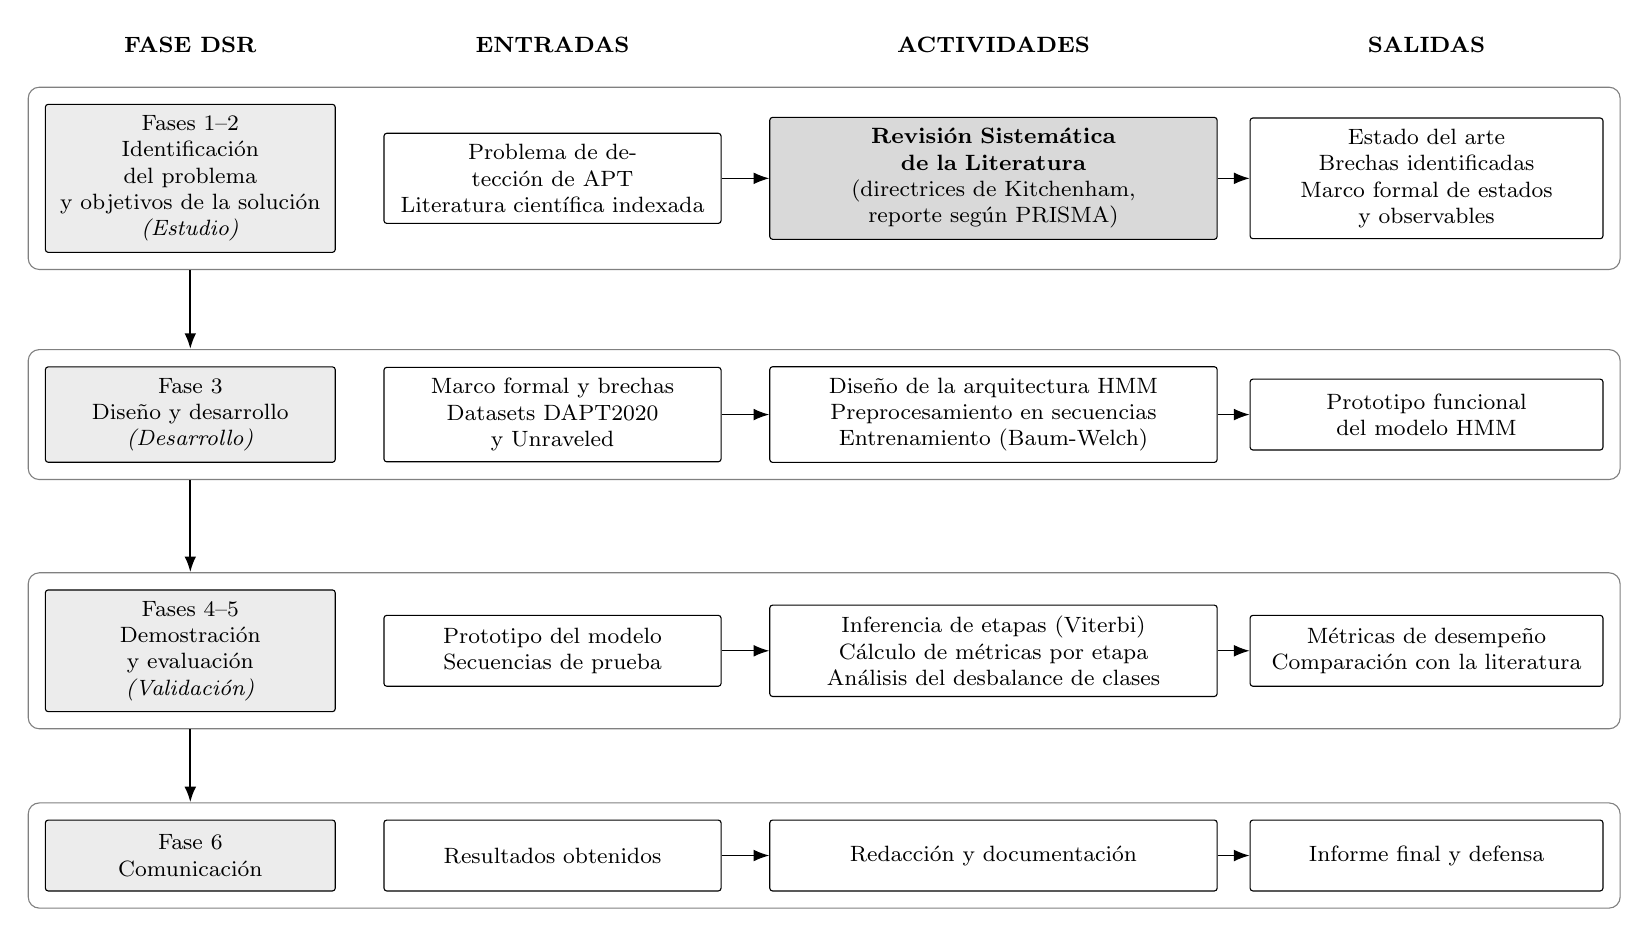
\begin{tikzpicture}[
    font=\footnotesize,
    box/.style={draw, rectangle, rounded corners=1pt, align=center, inner sep=4pt, minimum height=9mm},
    fase/.style={box, fill=gray!15, text width=3.4cm},
    ent/.style={box, fill=white, text width=4.0cm},
    act/.style={box, fill=white, text width=5.4cm},
    sal/.style={box, fill=white, text width=4.2cm},
    slr/.style={box, fill=gray!30, text width=5.4cm},
    fl/.style={-{Latex[length=2mm]}, thin}
]
 
\node at (0,1.1) {\bfseries FASE DSR};
\node at (4.6,1.1) {\bfseries ENTRADAS};
\node at (10.2,1.1) {\bfseries ACTIVIDADES};
\node at (15.7,1.1) {\bfseries SALIDAS};
 
% --- Bloque 1: Estudio ---
\node[fase] (f1) at (0,-0.6) {Fases 1--2\\Identificación del problema\\y objetivos de la solución\\\textit{(Estudio)}};
\node[ent]  (e1) at (4.6,-0.6) {Problema de detección de APT\\Literatura científica indexada};
\node[slr]  (a1) at (10.2,-0.6) {\textbf{Revisión Sistemática de la Literatura}\\(directrices de Kitchenham,\\reporte según PRISMA)};
\node[sal]  (s1) at (15.7,-0.6) {Estado del arte\\Brechas identificadas\\Marco formal de estados\\y observables};
\draw[fl] (e1) -- (a1);
\draw[fl] (a1) -- (s1);
\begin{scope}[on background layer]
\node[draw, gray, rounded corners, fit=(f1)(e1)(a1)(s1), inner sep=6pt] (b1) {};
\end{scope}
 
% --- Bloque 2: Desarrollo ---
\node[fase] (f2) at (0,-3.6) {Fase 3\\Diseño y desarrollo\\\textit{(Desarrollo)}};
\node[ent]  (e2) at (4.6,-3.6) {Marco formal y brechas\\Datasets DAPT2020 y Unraveled};
\node[act]  (a2) at (10.2,-3.6) {Diseño de la arquitectura HMM\\Preprocesamiento en secuencias\\Entrenamiento (Baum-Welch)};
\node[sal]  (s2) at (15.7,-3.6) {Prototipo funcional\\del modelo HMM};
\draw[fl] (e2) -- (a2);
\draw[fl] (a2) -- (s2);
\begin{scope}[on background layer]
\node[draw, gray, rounded corners, fit=(f2)(e2)(a2)(s2), inner sep=6pt] (b2) {};
\end{scope}
 
% --- Bloque 3: Validación ---
\node[fase] (f3) at (0,-6.6) {Fases 4--5\\Demostración y evaluación\\\textit{(Validación)}};
\node[ent]  (e3) at (4.6,-6.6) {Prototipo del modelo\\Secuencias de prueba};
\node[act]  (a3) at (10.2,-6.6) {Inferencia de etapas (Viterbi)\\Cálculo de métricas por etapa\\Análisis del desbalance de clases};
\node[sal]  (s3) at (15.7,-6.6) {Métricas de desempeño\\Comparación con la literatura};
\draw[fl] (e3) -- (a3);
\draw[fl] (a3) -- (s3);
\begin{scope}[on background layer]
\node[draw, gray, rounded corners, fit=(f3)(e3)(a3)(s3), inner sep=6pt] (b3) {};
\end{scope}
 
% --- Bloque 4: Comunicación ---
\node[fase] (f4) at (0,-9.2) {Fase 6\\Comunicación};
\node[ent]  (e4) at (4.6,-9.2) {Resultados obtenidos};
\node[act]  (a4) at (10.2,-9.2) {Redacción y documentación};
\node[sal]  (s4) at (15.7,-9.2) {Informe final y defensa};
\draw[fl] (e4) -- (a4);
\draw[fl] (a4) -- (s4);
\begin{scope}[on background layer]
\node[draw, gray, rounded corners, fit=(f4)(e4)(a4)(s4), inner sep=6pt] (b4) {};
\end{scope}
 
% flechas entre bloques
\draw[fl, thick] (b1.south -| f1) -- (b2.north -| f1);
\draw[fl, thick] (b2.south -| f2) -- (b3.north -| f2);
\draw[fl, thick] (b3.south -| f3) -- (b4.north -| f3);
 
\end{tikzpicture}%
}
\caption{Esquema integrado de la metodología de investigación. Fuente: Elaboración propia.}
\label{fig:dsr}
\end{figure}
\FloatBarrier

\section{Diseño de la revisión}

La Figura~\ref{fig:metodologia} desglosa el procedimiento interno de la revisión sistemática, correspondiente a la actividad central de las Fases 1 y 2 del esquema anterior. Mientras la Figura~\ref{fig:dsr} representa el ciclo completo de la investigación, esta detalla las tres etapas consecutivas en que se organiza la revisión (planificación, ejecución y reporte) junto con las herramientas empleadas en cada una. La primera etapa contempla la formulación de las preguntas de investigación y la definición de los criterios de inclusión y exclusión, cuyo resultado es un protocolo de revisión que fija las reglas antes de consultar cualquier base de datos. La segunda etapa corresponde a la ejecución de las ecuaciones de búsqueda sobre las fuentes seleccionadas y al cribado progresivo de los registros recuperados, procedimiento documentado mediante el diagrama de flujo PRISMA hasta obtener el corpus final. La tercera etapa se enfoca en la extracción, clasificación y síntesis de la información contenida en los estudios incluidos, con el fin de comparar los enfoques reportados en la literatura e identificar las brechas que fundamentan la propuesta.

\begin{figure}[h!]
\centering
\resizebox{\textwidth}{!}{%
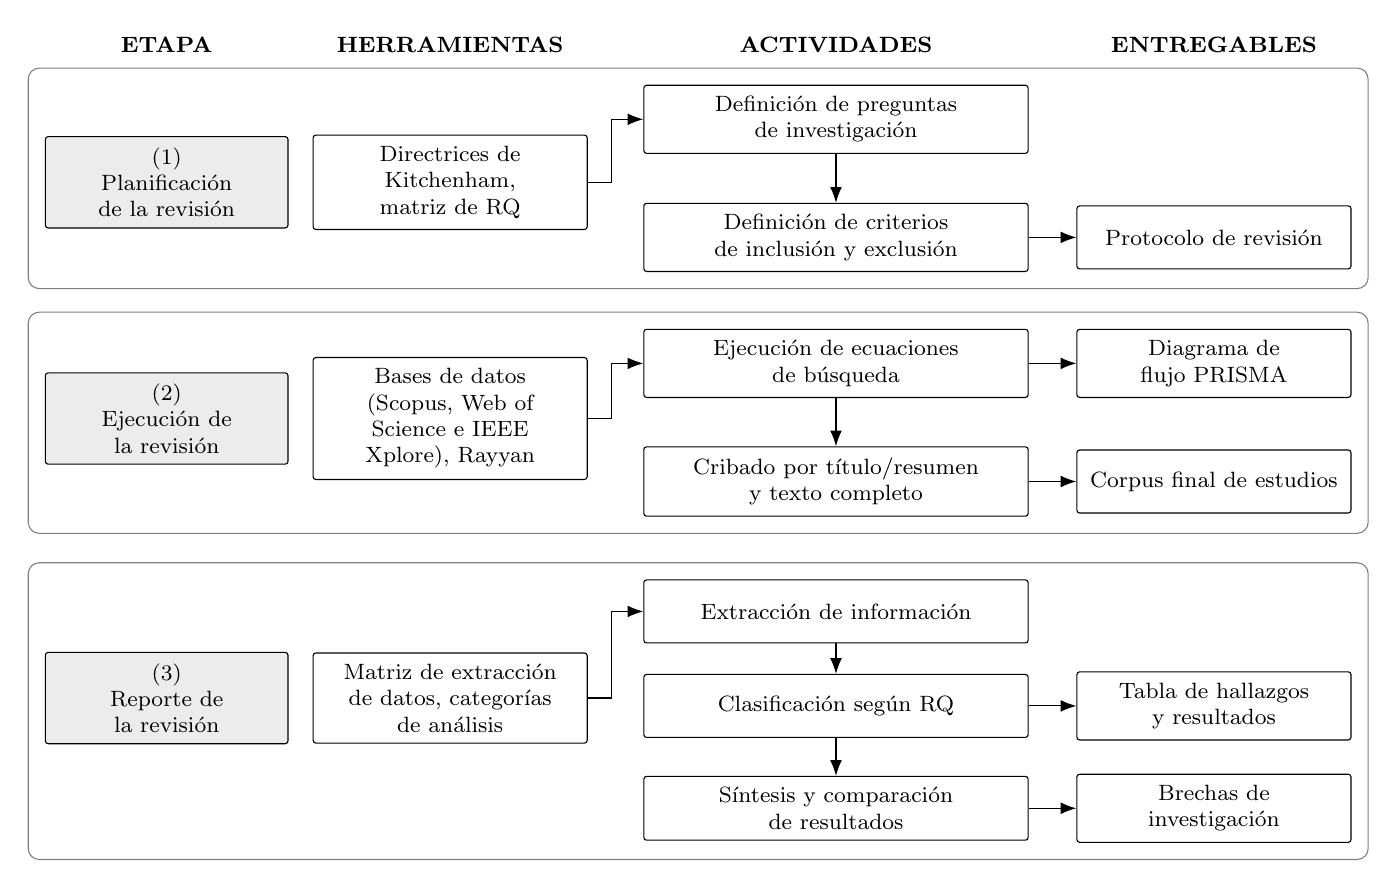
\begin{tikzpicture}[
    font=\footnotesize,
    box/.style={draw, rectangle, rounded corners=1pt, align=center, inner sep=4pt, minimum height=8mm},
    etapa/.style={box, fill=gray!15, text width=2.8cm},
    herr/.style={box, fill=white, text width=3.2cm},
    act/.style={box, fill=white, text width=4.6cm},
    ent/.style={box, fill=white, text width=3.2cm},
    flecha/.style={-{Latex[length=2mm]}, thin}
]
\node (h1) at (0,0.9) {\bfseries ETAPA};
\node (h2) at (3.6,0.9) {\bfseries HERRAMIENTAS};
\node (h3) at (8.5,0.9) {\bfseries ACTIVIDADES};
\node (h4) at (13.3,0.9) {\bfseries ENTREGABLES};

\node[etapa] (e1) at (0,-0.85) {(1)\\Planificación\\de la revisión};
\node[herr]  (t1) at (3.6,-0.85) {Directrices de\\Kitchenham,\\matriz de RQ};
\node[act]   (a1a) at (8.5,-0.05) {Definición de preguntas\\de investigación};
\node[act]   (a1b) at (8.5,-1.55) {Definición de criterios de inclusión y exclusión};
\node[ent]   (d1) at (13.3,-1.55) {Protocolo de revisión};
%\draw[flecha] (e1) -- (t1);
\draw[flecha] (t1.east) -- ++(0.3,0) |- (a1a.west);
\draw[flecha] (a1a) -- (a1b);
\draw[flecha] (a1b) -- (d1);
\begin{scope}[on background layer]
\node[draw, gray, rounded corners, fit=(e1)(t1)(a1a)(a1b)(d1), inner sep=6pt] {};
\end{scope}

\node[etapa] (e2) at (0,-3.85) {(2)\\Ejecución de\\la revisión};
\node[herr]  (t2) at (3.6,-3.85) {Bases de datos\\(Scopus, Web of Science e IEEE Xplore), Rayyan};
\node[act]   (a2a) at (8.5,-3.15) {Ejecución de ecuaciones\\de búsqueda};
\node[act]   (a2b) at (8.5,-4.65) {Cribado por título/resumen y texto completo};
\node[ent]   (d2a) at (13.3,-3.15) {Diagrama de flujo PRISMA};
\node[ent]   (d2b) at (13.3,-4.65) {Corpus final de estudios};
%\draw[flecha] (e2) -- (t2);
\draw[flecha] (t2.east) -- ++(0.3,0) |- (a2a.west);
\draw[flecha] (a2a) -- (a2b);
\draw[flecha] (a2a) -- (d2a);
\draw[flecha] (a2b) -- (d2b);
\begin{scope}[on background layer]
\node[draw, gray, rounded corners, fit=(e2)(t2)(a2a)(a2b)(d2a)(d2b), inner sep=6pt] {};
\end{scope}

\node[etapa] (e3) at (0,-7.4) {(3)\\Reporte de\\la revisión};
\node[herr]  (t3) at (3.6,-7.4) {Matriz de extracción\\de datos, categorías\\de análisis};
\node[act]   (a3a) at (8.5,-6.3) {Extracción de información};
\node[act]   (a3b) at (8.5,-7.5) {Clasificación según RQ};
\node[act]   (a3c) at (8.5,-8.8) {Síntesis y comparación\\de resultados};
\node[ent]   (d3a) at (13.3,-7.5) {Tabla de hallazgos\\y resultados};
\node[ent]   (d3b) at (13.3,-8.8) {Brechas de\\investigación};
%\draw[flecha] (e3) -- (t3);
\draw[flecha] (t3.east) -- ++(0.3,0) |- (a3a.west);
\draw[flecha] (a3a) -- (a3b);
\draw[flecha] (a3b) -- (a3c);
\draw[flecha] (a3b) -- (d3a);
\draw[flecha] (a3c) -- (d3b);
\begin{scope}[on background layer]
\node[draw, gray, rounded corners, fit=(e3)(t3)(a3a)(a3b)(a3c)(d3a)(d3b), inner sep=6pt] {};
\end{scope}
\end{tikzpicture}%
}
\caption{Etapas de la revisión sistemática de la literatura. Fuente: Elaboración propia.}
\label{fig:metodologia}
\end{figure}
\FloatBarrier

\section{Preguntas de investigación}

Para guiar el proceso de revisión y asegurar coherencia con los objetivos del proyecto, se definieron cuatro preguntas de investigación, cada una asociada a una ecuación de búsqueda propia (Tabla~\ref{tab:rqs}).

La formulación de las preguntas de investigación siguió la estructura PICOC recomendada por Kitchenham y Charters \parencite{kitchenham2007guidelines}, considerando como población las campañas de Amenazas Persistentes Avanzadas, como intervención los modelos probabilísticos aplicados a su detección, y como resultados las características, limitaciones y desempeño reportados. El criterio de comparación no se define de forma explícita, dado el carácter exploratorio de la revisión, orientada a caracterizar el estado del conocimiento antes que a contrastar dos tratamientos específicos. El contexto corresponde a entornos de red organizacionales.

\begin{table}[h!]
\centering
\small
\caption{Preguntas de investigación de la revisión sistemática.}
\label{tab:rqs}
\begin{tabular}{p{1.2cm} p{14.4cm}}
\hline
\textbf{ID} & \textbf{Pregunta de investigación} \\
\hline
RQ1 & ¿Qué modelos probabilísticos se han aplicado a la detección de Amenazas Persistentes Avanzadas, y cuáles son sus principales características? \\
RQ2 & ¿Cómo se han aplicado específicamente los Modelos Ocultos de Markov (HMM) a la detección o predicción de APT, y qué variantes se han utilizado? \\
RQ3 & ¿Qué datasets se han utilizado para entrenar y validar estos modelos, y qué limitaciones presentan? \\
RQ4 & ¿Qué estrategias existen para abordar el desbalance de clases en la detección de amenazas, y cómo afectan el desempeño de los modelos? \\
\hline
\end{tabular}
\end{table}
\FloatBarrier

La RQ1 busca caracterizar el panorama general de enfoques probabilísticos aplicados al problema, estableciendo una base comparativa que permita situar la propuesta dentro de una familia de técnicas más amplia. La RQ2 profundiza en los Modelos Ocultos de Markov, identificando cómo se han definido los estados ocultos y las variables observables en trabajos previos, así como las variantes empleadas y sus resultados. Por su parte, la RQ3 se orienta a los conjuntos de datos disponibles para la validación empírica, atendiendo tanto a su representatividad respecto de campañas APT reales como a sus limitaciones documentadas. Finalmente, la RQ4 aborda el desbalance de clases, condición inherente a los escenarios de detección de amenazas, con el fin de identificar qué estrategias de mitigación se han probado y qué efecto tienen sobre el desempeño de los modelos.

\section{Criterios de inclusión y exclusión}

Para asegurar la relevancia y calidad de los estudios seleccionados, se definieron los siguientes criterios:

\begin{table}[h!]
\centering
\small
\caption{Criterios de inclusión.}
\label{tab:inclusion}
\begin{tabular}{p{1.2cm} p{14.4cm}}
\hline
\textbf{ID} & \textbf{Criterio de Inclusión (CI)} \\
\hline
CI-1 & Abordan la detección o predicción de Amenazas Persistentes Avanzadas o ataques multi-etapa. \\
CI-2 & Emplean modelos probabilísticos, con especial atención a enfoques basados en Modelos de Markov. \\
CI-3 & Presentan validación empírica sobre datos, mediante experimentación o métricas cuantitativas. \\
CI-4 & Publicados desde 2011, año de formalización del modelo de \textit{kill chain} de intrusión. Se exceptúan los estudios asociados a la RQ4, dado que la literatura sobre desbalance de clases es anterior a esa fecha y cuenta con trabajos seminales previos. \\
CI-5 & Publicados en fuentes académicas con revisión por pares. Se exceptúan los reportes técnicos fundacionales ampliamente citados en el área, dado su rol como referencia seminal. \\
CI-6 & Publicaciones en inglés o español. \\
CI-7 & Correspondientes a artículos de revista, \textit{proceedings} de conferencias o capítulos de libro. \\
CI-8 & Texto completo disponible mediante acceso institucional o abierto. \\
\hline
\end{tabular}
\end{table}
\FloatBarrier

\begin{table}[h!]
\centering
\small
\caption{Criterios de exclusión.}
\label{tab:exclusion}
\begin{tabular}{p{1.2cm} p{14.4cm}}
\hline
\textbf{ID} & \textbf{Criterio de Exclusión (CE)} \\
\hline
CE-1 & No alineados con la detección de amenazas en sistemas o redes computacionales. \\
CE-2 & Estudios puramente teóricos sobre modelos probabilísticos, sin aplicación al dominio de la seguridad. \\
CE-3 & Registros duplicados identificados en múltiples fuentes. Ante versiones múltiples de una misma investigación, se conserva la más completa o reciente. \\
CE-4 & Publicaciones no académicas o sin proceso de revisión por pares, salvo la excepción indicada en el criterio CI-5. \\
CE-5 & Detección de amenazas basada en eventos aislados, sin componente secuencial o multi-etapa, por no aportar a la modelación de la progresión de un ataque. \\
CE-6 & Sin disponibilidad del texto completo. \\
CE-7 & Revisiones sistemáticas de literatura (SLR) previas. Estas pueden citarse como contexto narrativo, pero no se extraen como estudio primario en la matriz de extracción de datos. \\
CE-8 & Estudios que, si bien abordan la detección de amenazas, no aportan evidencia relevante a ninguna de las preguntas de investigación formuladas: emplean conjuntos de datos de intrusiones genéricos sin etiquetado por etapas de ataque, o no describen ni discuten las características de los datos utilizados. \\
\hline
\end{tabular}
\end{table}
\FloatBarrier

Cabe señalar una excepción respecto del criterio CI-5: se admite la inclusión de reportes técnicos fundacionales ampliamente citados en el área, como el trabajo de Hutchins et al. \parencite{hutchins2011killchain}, dado su carácter de referencia seminal para la caracterización por etapas de las campañas APT.

\section{Fuentes de información y estrategia de búsqueda}

La búsqueda sistemática considera tres fuentes de información científica seleccionadas por su cobertura en ciencias de la computación y ciberseguridad, y por su disponibilidad mediante acceso institucional: Scopus, Web of Science e IEEE Xplore. Las dos primeras corresponden a bases de datos de indexación multidisciplinar que agregan contenido de las principales editoriales del área (incluidas ACM, Springer, Elsevier y Wiley), mientras que IEEE Xplore se incorpora de forma complementaria dada la concentración de literatura especializada en detección de intrusiones presente en sus publicaciones.

Para garantizar una adecuada correspondencia entre los objetivos del estudio y la evidencia recuperada, se definió una ecuación de búsqueda específica para cada pregunta de investigación, evitando el uso de una única consulta general replicada en todas las bases de datos. Esta decisión permite capturar con mayor precisión los conceptos particulares abordados por cada pregunta. Asimismo, todas las búsquedas se aplicaron sobre los campos de título, resumen y palabras clave, dado que restringirlas únicamente al título excluiría trabajos cuya contribución metodológica solo se explicita en el resumen. Las ecuaciones utilizadas se presentan en la Tabla~\ref{tab:ecuaciones}.

\begin{table}[h!]
\centering
\small
\caption{Ecuaciones de búsqueda por pregunta de investigación.}
\label{tab:ecuaciones}
\begin{tabular}{c p{9.4cm} c c c c}
\hline
\textbf{RQ} & \textbf{Ecuación de búsqueda} & \textbf{Scopus} & \textbf{WoS} & \textbf{IEEE} & \textbf{Total} \\
\hline
RQ1 & \textit{("advanced persistent threat*" OR APT OR "multi-stage attack*" OR "multi-step attack*") AND ("probabilistic model*" OR "Bayesian network*" OR "Markov model*" OR "stochastic model*" OR "probabilistic approach*") AND (detect* OR predict* OR classif*)} & 127 & 67 & 85 & 279 \\
\hline
RQ2 & \textit{("advanced persistent threat*" OR APT OR "attack campaign*" OR "kill chain" OR "multi-stage attack*") AND ("hidden Markov model*" OR HMM OR "Markov chain*" OR "hidden semi-Markov*") AND (detect* OR predict* OR model* OR classif*)} & 103 & 27 & 80 & 210 \\
\hline
RQ3 & \textit{("advanced persistent threat*" OR APT OR "multi-stage attack*") AND (dataset* OR benchmark* OR corpus) AND ("machine learning" OR "deep learning" OR classif*)} & 279 & 154 & 40 & 473 \\
\hline
RQ4 & \textit{("class imbalance*" OR "imbalanced data*" OR SMOTE) AND ("intrusion detection" OR "threat detection" OR "anomaly detection") AND ("advanced persistent threat*" OR APT OR "multi-stage attack*")} & 47 & 19 & 48 & 114 \\
\hline
\multicolumn{2}{r}{\textbf{Total de registros identificados}} & 556 & 267 & 253 & 1076 \\
\hline
\end{tabular}

\vspace{2mm}

\vspace{2mm}
\begin{minipage}{\textwidth}
\small
\textit{Nota:} Las ecuaciones se presentan en su forma genérica. Su sintaxis específica varía según la plataforma: \texttt{TITLE-ABS-KEY(...)} en Scopus, \texttt{TS=(...)} en Web of Science y el campo \textit{All Metadata} en IEEE Xplore. En esta última, la ecuación de RQ1 omite el término \textit{"probabilistic approach*"} debido a la restricción de la plataforma, que admite un máximo de diez comodines por consulta. El criterio temporal establecido en CI-4 se aplicó mediante el operador \texttt{PUBYEAR} en Scopus y mediante los filtros propios de cada plataforma en Web of Science e IEEE Xplore. La ecuación de RQ4 no incorpora restricción temporal, conforme a la excepción prevista en dicho criterio.
\end{minipage}

\end{table}
\FloatBarrier


\section{Proceso de selección de estudios}

El proceso de selección se ejecutó siguiendo las cuatro etapas del modelo PRISMA 2020, cuyo resultado se sintetiza en la Figura~\ref{fig:prisma}. La búsqueda inicial recuperó 1.076 registros, distribuidos entre Scopus (556), Web of Science (267) e IEEE Xplore (253). Tras la eliminación de 473 duplicados, atribuibles al solapamiento entre las bases de datos consultadas y entre las ecuaciones asociadas a cada pregunta de investigación, se sometieron 603 registros al cribado por título y resumen.

En esta etapa se excluyeron 311 registros. La causa predominante correspondió al criterio CE-8, aplicado a estudios que, pese a situarse en el dominio de la detección de amenazas, no aportaban evidencia relevante respecto de las preguntas formuladas. Un número significativo de exclusiones bajo el criterio CE-1 se originó en coincidencias léxicas espurias, derivadas de la coincidencia de la sigla APT con fragmentos de términos como \textit{adaptive} o \textit{adaptation}, así como con su acepción en otras disciplinas.

De los 292 artículos que avanzaron a la evaluación de texto completo, 199 debieron ser excluidos por no disponerse de acceso al documento completo (CE-6) y 10 por corresponder a dominios ajenos al objeto de estudio (CE-1). El corpus final quedó constituido por 83 estudios primarios, de los cuales 16 emplean modelos de Markov, 18 abordan explícitamente el desbalance de clases y 6 utilizan los conjuntos de datos seleccionados para este trabajo.

\begin{figure}[h!]
\centering
\resizebox{0.95\textwidth}{!}{%
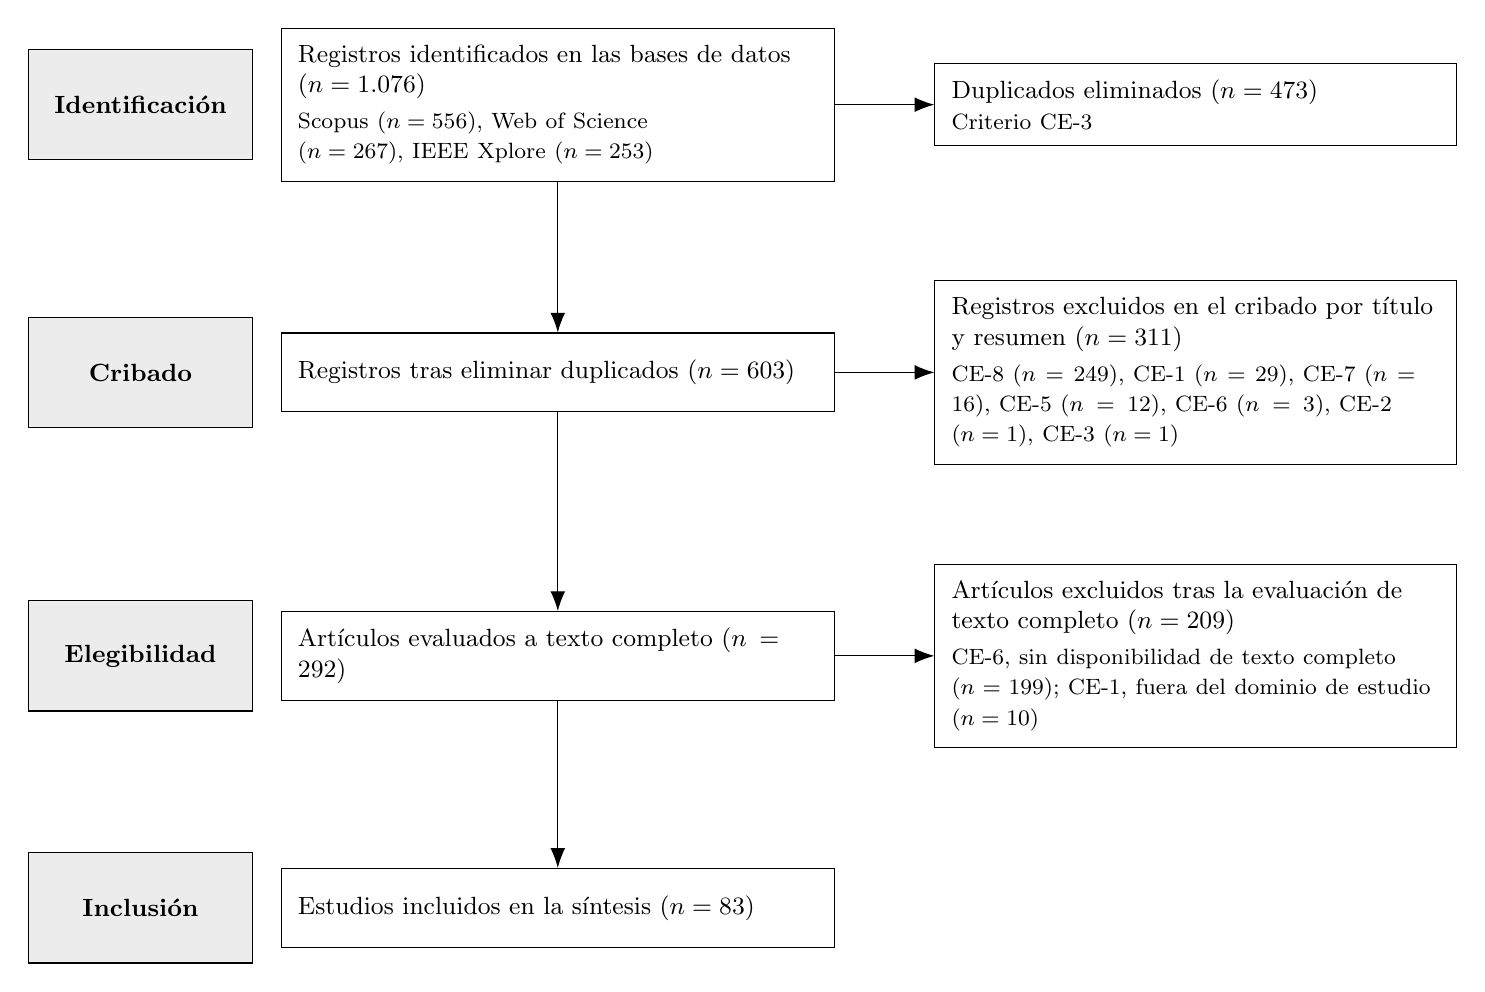
\begin{tikzpicture}[
    font=\small,
    caja/.style={draw, rectangle, align=left, inner sep=6pt, text width=6.6cm, minimum height=10mm},
    exc/.style={draw, rectangle, align=left, inner sep=6pt, text width=6.2cm, minimum height=10mm},
    etapa/.style={draw, rectangle, fill=gray!15, align=center, inner sep=5pt, text width=2.5cm, minimum height=14mm},
    fl/.style={-{Latex[length=2.5mm]}, thin}
]
 
\node[etapa] (l1) at (-4.8,0)    {\textbf{Identificación}};
\node[etapa] (l2) at (-4.8,-3.4) {\textbf{Cribado}};
\node[etapa] (l3) at (-4.8,-7.0) {\textbf{Elegibilidad}};
\node[etapa] (l4) at (-4.8,-10.2){\textbf{Inclusión}};
 
\node[caja] (c1) at (0.5,0) {Registros identificados en las bases de datos ($n = 1{.}076$)\\[2pt]
\footnotesize Scopus ($n=556$), Web of Science \newline ($n=267$), IEEE Xplore ($n=253$)};
 
\node[caja] (c2) at (0.5,-3.4) {Registros tras eliminar duplicados ($n = 603$)};
 
\node[caja] (c3) at (0.5,-7.0) {Artículos evaluados a texto completo ($n = 292$)};
 
\node[caja] (c4) at (0.5,-10.2) {Estudios incluidos en la síntesis ($n = 83$)};
 
\node[exc] (e1) at (8.6,0) {Duplicados eliminados ($n = 473$)\\
\footnotesize Criterio CE-3};
 
\node[exc] (e2) at (8.6,-3.4) {Registros excluidos en el cribado por título y resumen ($n = 311$)\\[2pt]
\footnotesize CE-8 ($n=249$), CE-1 ($n=29$), CE-7 ($n=16$), CE-5 ($n=12$), CE-6 ($n=3$), CE-2 ($n=1$), CE-3 ($n=1$)};
 
\node[exc] (e3) at (8.6,-7.0) {Artículos excluidos tras la evaluación de texto completo ($n = 209$)\\[2pt]
\footnotesize CE-6, sin disponibilidad de texto completo ($n=199$); CE-1, fuera del dominio de estudio ($n=10$)};
 
\draw[fl] (c1) -- (c2);
\draw[fl] (c2) -- (c3);
\draw[fl] (c3) -- (c4);
 
\draw[fl] (c1.east) -- (e1.west);
\draw[fl] (c2.east) -- (e2.west);
\draw[fl] (c3.east) -- (e3.west);
 
\end{tikzpicture}%
}
\caption{Diagrama de flujo del proceso de selección de estudios, según la declaración PRISMA 2020. Fuente: Elaboración propia.}
\label{fig:prisma}
\end{figure}

\section{Categorías de análisis}

Con el propósito de orientar sistemáticamente el análisis de la literatura recopilada, se definió un conjunto de categorías derivadas directamente de las preguntas de investigación. Esta estructura permite clasificar la información extraída de cada estudio de forma coherente con los objetivos del proyecto y facilita la comparación entre enfoques.

\begin{table}[h!]
\centering
\small
\caption{Categorías y subcategorías de análisis.}
\begin{tabular}{p{1.0cm} p{4.6cm} p{9.6cm}}
\hline
\textbf{RQ} & \textbf{Categoría} & \textbf{Subcategorías} \\
\hline
RQ1 & C1. Modelos probabilísticos & Redes bayesianas, grafos de ataque bayesianos, modelos \newline estocásticos \\
RQ2 & C2. Modelos de Markov & Definición de estados ocultos, variables observables, \newline algoritmos de entrenamiento e inferencia \\
RQ3 & C3. Conjuntos de datos & Representatividad de campañas APT, etapas etiquetadas, \newline limitaciones documentadas \\
RQ4 & C4. Desbalance de clases & Estrategias de sobremuestreo, submuestreo, métricas robustas al desbalance \\
\hline
\end{tabular}
\end{table}
\FloatBarrier

A partir de este esquema, cada estudio incluido se registra en la matriz de extracción de datos indicando el modelo empleado, el conjunto de datos utilizado, las métricas reportadas y las limitaciones declaradas por sus autores, junto con la categoría o categorías a las que responde. Este procedimiento permite construir de manera sistemática el Estado del Arte y sustentar la identificación de brechas que fundamentan la propuesta desarrollada en este trabajo.

\subsection{Evaluación del riesgo de sesgo y extracción de evidencia}
De manera análoga a los estudios secundarios en ciberseguridad empírica, no se aplicó una herramienta estandarizada de sesgo clínico (como RoB 2 o Newcastle-Ottawa), debido a la naturaleza estrictamente técnica, experimental y computacional de los estudios analizados. La heterogeneidad de métricas, conjuntos de datos propietarios y topologías de red en la literatura dificulta el uso de escalas cuantitativas universales de sesgo.

En su lugar, la validez interna y reproducibilidad de la revisión se resguardó mediante tres mecanismos operativos:
\begin{enumerate}
    \item \textbf{Filtrado por pares e impacto:} Restricción a fuentes con revisión por pares indexadas en Scopus, Web of Science e IEEE Xplore, exigiendo un umbral mínimo de tres citas (CI-8) para publicaciones anteriores a 2025.
    \item \textbf{Verificación de consistencia cruzada en extracción:} Cada estudio del corpus final ($n=83$) fue analizado mediante una matriz estructurada que desagrega explícitamente: 
    \begin{itemize}
        \item Familia del modelo probabilístico.
        \item Definición formal de estados y observaciones.
        \item Dataset utilizado.
        \item Métricas reportadas.
        \item Tratamiento del desbalance de datos.
    \end{itemize}
    \item \textbf{Control de sesgo de reporte de métricas:} Se contrastó sistemáticamente la disparidad entre exactitud global (\textit{Accuracy}) y métricas sensibles a la clase minoritaria ($F_1$-score y \textit{Recall}), permitiendo aislar publicaciones con evaluaciones sobredimensionadas debidas al desbalance de clases.
\end{enumerate}
\chapter{Estado del Arte}

Con el propósito de caracterizar el estado actual de la investigación sobre modelos probabilísticos aplicados a la detección de Amenazas Persistentes Avanzadas, esta sección presenta la síntesis y el análisis de los estudios seleccionados mediante el proceso de revisión sistemática descrito previamente. El análisis se estructura en función de las preguntas de investigación definidas, lo que permite examinar los enfoques empleados, los conjuntos de datos utilizados y las estrategias adoptadas frente al desbalance de clases. A partir de la evidencia recopilada se identifican tendencias, fortalezas y limitaciones de las soluciones existentes, así como las brechas que fundamentan la propuesta presentada en este trabajo.

\section{Panorama bibliométrico del corpus}

El corpus final quedó constituido por 77 estudios primarios, de los cuales 70 corresponden a artículos de revista y 7 a comunicaciones en conferencias. La revista IEEE Access concentra la mayor proporción de publicaciones del corpus, con 17 estudios, seguida por IEEE Transactions on Dependable and Secure Computing.

La distribución temporal, presentada en la Figura~\ref{fig:temporal}, evidencia un crecimiento sostenido del interés investigativo en el área. Mientras que entre 2017 y 2022 la producción se mantuvo en un rango de tres a ocho estudios anuales, a partir de 2023 se observa una expansión marcada, que alcanza 22 estudios en 2026. Más de la mitad del corpus corresponde a publicaciones de los últimos tres años, lo que confirma que se trata de un área de investigación activa y en desarrollo, y no de un campo consolidado con soluciones establecidas.

\begin{figure}[h!]
\centering
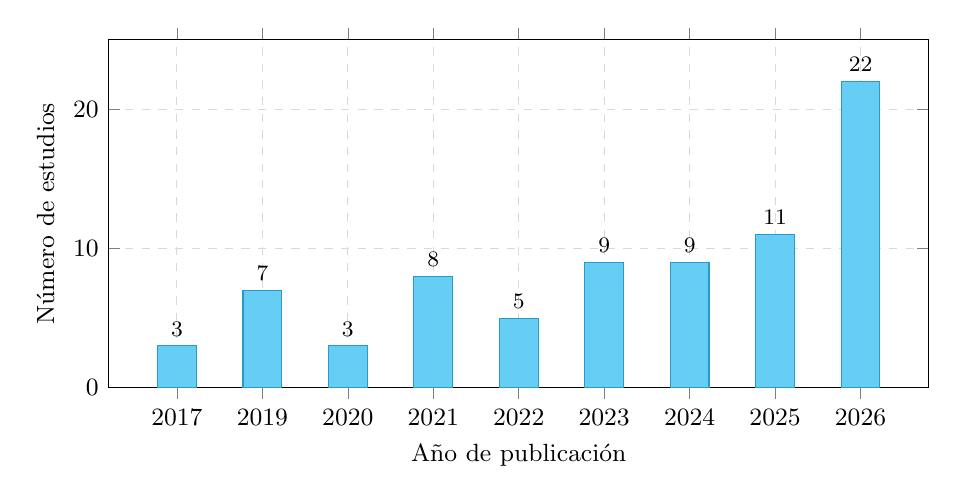
\begin{tikzpicture}
\begin{axis}[
    width=12cm, height=6cm,
    ybar, bar width=14pt,
    ymin=0, ymax=25,
    symbolic x coords={2017,2019,2020,2021,2022,2023,2024,2025,2026},
    xtick=data,
    ylabel={Número de estudios},
    xlabel={Año de publicación},
    nodes near coords, nodes near coords style={font=\footnotesize},
    grid=major, grid style={dashed,gray!30},
    tick label style={font=\small}, label style={font=\small},
]
\addplot[fill=cyan!60,draw=cyan!80!black] coordinates {(2017,3)(2019,7)(2020,3)(2021,8)(2022,5)(2023,9)(2024,9)(2025,11)(2026,22)};
\end{axis}
\end{tikzpicture}
\caption{Distribución temporal de los estudios del corpus (2017--2026). Fuente: Elaboración propia.}
\label{fig:temporal}
\end{figure}

La Figura~\ref{fig:modelos} presenta la distribución de los estudios según la familia de modelos que mencionan en su texto completo, conforme a la Tabla~\ref{tab:hallazgos}. Los enfoques basados en aprendizaje profundo constituyen el grupo más numeroso, con 60 estudios, seguidos por las técnicas clásicas de aprendizaje automático con 48 y los modelos de Markov con 32, de los cuales 19 corresponden a Modelos Ocultos de Markov. Los modelos basados en grafos, redes bayesianas y teoría de juegos presentan una participación menor pero significativa. Cabe señalar que un mismo estudio puede emplear o discutir más de una familia de modelos, por lo que las categorías no son mutuamente excluyentes.

\begin{figure}[h!]
\centering
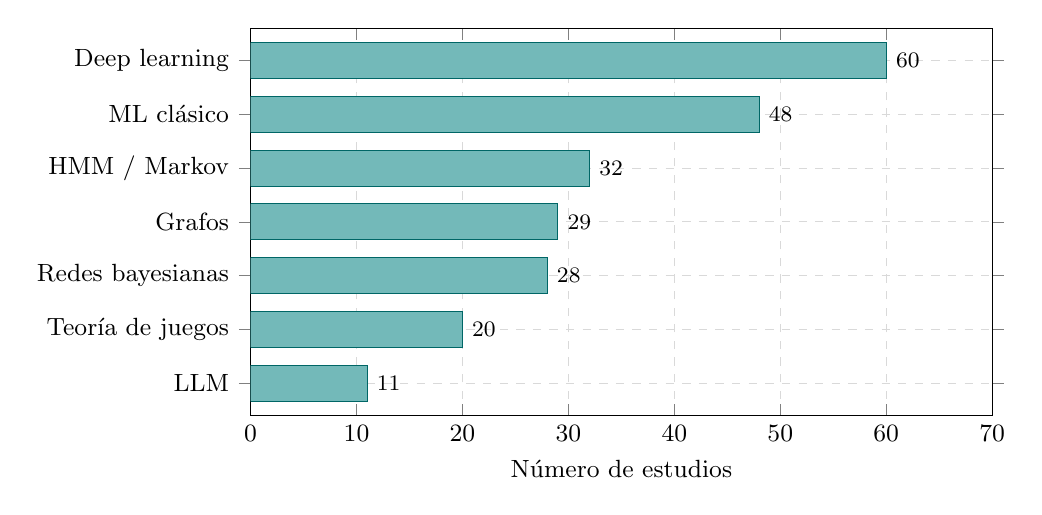
\begin{tikzpicture}
\begin{axis}[
    width=11cm, height=6.5cm,
    xbar, bar width=13pt,
    xmin=0, xmax=70,
    symbolic y coords={LLM,Teoría de juegos,Redes bayesianas,Grafos,HMM / Markov,ML clásico,Deep learning},
    ytick=data,
    xlabel={Número de estudios},
    nodes near coords, nodes near coords style={font=\footnotesize},
    grid=major, grid style={dashed,gray!30},
    tick label style={font=\small}, label style={font=\small},
]
\addplot[fill=teal!55,draw=teal!80!black] coordinates {(11,LLM)(20,Teoría de juegos)(28,Redes bayesianas)(29,Grafos)(32,HMM / Markov)(48,ML clásico)(60,Deep learning)};
\end{axis}
\end{tikzpicture}
\caption{Familias de modelos empleadas en los estudios del corpus. Fuente: Elaboración propia.}
\label{fig:modelos}
\end{figure}

\section{Hallazgos por categoría de análisis}

Esta sección presenta el análisis organizado según las categorías definidas en la metodología. La Tabla~\ref{tab:hallazgos} identifica, para cada estudio del corpus, las familias de modelos empleadas, los conjuntos de datos utilizados y el tratamiento explícito del desbalance de clases.

La revisión de los textos completos permite precisar la caracterización del corpus. Treinta y dos estudios mencionan modelos de Markov en alguna de sus variantes, de los cuales diecinueve refieren específicamente Modelos Ocultos de Markov. Nueve estudios trabajan con DAPT2020 y nueve con Unraveled, cifras superiores a las que sugería el análisis de resúmenes, lo que indica que una proporción relevante de los trabajos no declara el conjunto de datos en dicha sección. Treinta y seis estudios abordan de manera explícita el desbalance de clases, cerca de la mitad del corpus. Cabe precisar que estas cifras corresponden a la presencia de los términos en el texto completo, por lo que incluyen tanto el uso efectivo como las referencias a trabajos previos.

\begin{footnotesize}
\setlength{\tabcolsep}{4pt}
\renewcommand{\arraystretch}{1.15}
\begin{xltabular}{\linewidth}{|p{3.3cm}|c|X|p{3.6cm}|c|}

\caption{Hallazgos por categoría de análisis en los estudios del corpus}
\label{tab:hallazgos} \\
\hline
\textbf{Estudio} & \textbf{Año} & \textbf{Modelos / Técnicas} & \textbf{Conjuntos de datos} & \textbf{Desb.} \\
\hline
\endfirsthead

\caption[]{Hallazgos por categoría de análisis en los estudios del corpus (Continuación)} \\
\hline
\textbf{Estudio} & \textbf{Año} & \textbf{Modelos / Técnicas} & \textbf{Conjuntos de datos} & \textbf{Desb.} \\
\hline
\endhead

\hline
\multicolumn{5}{|r|}{\textit{Continúa en la siguiente página\dots}} \\ \hline
\endfoot

\hline
\endlastfoot


Açıkgözoğlu \parencite{acikgozoglu_explainable_2026}& 2026 & Deep L., ML clás., Juegos & ToN-IoT & x \\
Alsubait \parencite{alsubait_large_2026} & 2026 & Markov, Grafos, Deep L., LLM & CICIDS, NSL-KDD & x \\
El Alami et al. \parencite{el_alami_real-time_2026} & 2026 & Deep L., ML clás., LLM & CICIDS, UNSW, KDD99 & x \\
Ferazza et al. \parencite{ferazza_logs_2026} & 2026 & Deep L., LLM & -- & x \\
Giacobbe et al. \parencite{giacobbe_enforcing_2026} & 2026 & Markov & -- &  \\
Hölbl y Rotovnik \parencite{holbl_machine_2026} & 2026 & Bayes, Grafos, Deep L., ML clás. & DAPT2020, Unraveled, DARPA, CICAPT, CICIDS, NSL-KDD, UNSW & x \\
Hussain y Petrova \parencite{hussain_threat_2026} & 2026 & Bayes, Deep L., ML clás., LLM & -- & x \\
Jiao et al. \parencite{jiao_bg-flipin_2026} & 2026 & Markov, Bayes, Juegos & -- &  \\
K et al. \parencite{k_advanced_2026} & 2026 & Bayes, Grafos, Deep L., ML clás. & DAPT2020, Unraveled, CICAPT, NSL-KDD, UNSW, ToN-IoT, KDD99 & x \\
Kumar et al. \parencite{kumar_hlpmmgrsphtru_2026} & 2026 & HMM, Deep L., ML clás. & CICIDS & x \\
Lahari et al. \parencite{lahari_intelligent_2026} & 2026 & Deep L., ML clás. & -- & x \\
M. U. Basharat et al. \parencite{m_u_basharat_advanced_2026} & 2026 & Deep L., ML clás. & KDD99 & x \\
P. Firdani et al. \parencite{p_firdani_multi-layer_2026} & 2026 & Grafos, Deep L., LLM & DARPA, CICAPT & x \\
Puccetti et al. \parencite{puccetti_capture_2026} & 2026 & Grafos, Deep L., ML clás. & DAPT2020, Unraveled, DARPA, OpTC, CICAPT, CICIDS, NSL-KDD, ToN-IoT, KDD99 & x \\
R. Alfageer et al. \parencite{r_alfageer_multi-stage_2026} & 2026 & Deep L., ML clás., LLM & CICIDS, NSL-KDD, UNSW, ToN-IoT & x \\
R. Huang \parencite{r_huang_efficient_2026} & 2026 & Deep L., ML clás. & -- & x \\
Salah et al. \parencite{salah_dual-model_2026} & 2026 & Grafos, Deep L., ML clás., LLM & CICAPT, CICIDS, UNSW, ToN-IoT & x \\
Shahzad et al. \parencite{shahzad_autonomous_2026} & 2026 & Markov, Deep L., ML clás. & CICIDS, NSL-KDD, UNSW, ToN-IoT &  \\
Sripada et al. \parencite{sripada_hybridml_2026} & 2026 & Bayes, Deep L., ML clás., Juegos & CICIDS, NSL-KDD, UNSW, ToN-IoT, KDD99 & x \\
Yilmaz et al. \parencite{yilmaz_non-local_2026} & 2026 & Bayes, Deep L., ML clás. & CICIDS, UNSW, ToN-IoT & x \\
You et al. \parencite{you_comparative_2026} & 2026 & Deep L., ML clás. & CICIDS, NSL-KDD, UNSW & x \\
Zhao et al. \parencite{zhao_alert-driven_2026} & 2026 & Bayes, Deep L., Juegos & -- &  \\
Bani Melhem et al. \parencite{bani_melhem_lens_2025} & 2025 & Deep L., ML clás., LLM & CICAPT & x \\
Benabderrahmane et al. \parencite{benabderrahmane_ranking-enhanced_2025} & 2025 & Grafos, Deep L., ML clás. & DARPA, CICIDS, NSL-KDD, UNSW, KDD99 & x \\
Cai et al. \parencite{cai_detecting_2025} & 2025 & Bayes, Grafos, Deep L., ML clás. & Unraveled & x \\
Chen y Yan \parencite{chen_research_2025} & 2025 & Deep L., ML clás. & -- & x \\
Chourasiya et al. \parencite{chourasiya_advanced_2025} & 2025 & Bayes, Deep L., ML clás., LLM & CICIDS, UNSW &  \\
Ibrahim et al. \parencite{ibrahim_optimized_2025} & 2025 & Deep L., ML clás. & DAPT2020, Unraveled, CICIDS, NSL-KDD, UNSW &  \\
L. Zhang \parencite{l_zhang_implementing_2025} & 2025 & Deep L., ML clás. & DARPA & x \\
Mittal et al. \parencite{mittal_proactive_2025} & 2025 & HMM, Markov, Grafos, Deep L., ML clás., Juegos & -- & x \\
Nicho et al. \parencite{nicho_enhanced_2025} & 2025 & HMM, Bayes, Deep L., ML clás. & -- & x \\
Rivas et al. \parencite{rivas_analysis_2025} & 2025 & Bayes, Deep L., ML clás., Juegos & DAPT2020, Unraveled & x \\
S. Lee et al. \parencite{s_lee_aptstop_2025} & 2025 & HMM, Bayes, Grafos, Deep L., ML clás., LLM, Juegos & DARPA &  \\
Byrapuneni y Saidireddy \parencite{byrapuneni_efficient_2024} & 2024 & Bayes, Deep L., ML clás. & DARPA, NSL-KDD, KDD99 & x \\
Cheng et al. \parencite{cheng_kairos_2024} & 2024 & Grafos, Deep L. & DARPA, OpTC &  \\
Erfan Mazaheri y Shameli-Sendi \parencite{erfan_mazaheri_aptracker_2024} & 2024 & Bayes, Deep L., ML clás. & -- & x \\
J. Jiao et al. \parencite{j_jiao_fpgaa_2024} & 2024 & Grafos, Deep L. & DARPA &  \\
Lo et al. \parencite{lo_digital_2024} & 2024 & Deep L. & -- &  \\
Ma et al. \parencite{ma_anomaly_2024} & 2024 & HMM, Markov, Bayes, Deep L., ML clás. & DARPA, CICIDS &  \\
Mamun et al. \parencite{mamun_limitations_2024} & 2024 & Bayes, Deep L., ML clás. & DAPT2020, Unraveled, DARPA, CICIDS, NSL-KDD, UNSW, KDD99 & x \\
Soliman et al.\parencite{soliman_rank_2024}  & 2024 & Grafos, Deep L. & DARPA, KDD99 &  \\
Zhang et al. \parencite{zhang_secaas-based_2024} & 2024 & Markov, Grafos, Deep L., Juegos & -- &  \\
Chen et al. \parencite{chen_machine_2023} & 2023 & Deep L., ML clás. & CICIDS, NSL-KDD, UNSW, ToN-IoT, KDD99 & x \\
Javed et al. \parencite{javed_apt_2023} & 2023 & HMM, Bayes, Deep L., ML clás., LLM, Juegos & DAPT2020, CICIDS, NSL-KDD & x \\
Kazeminajafabadi y Imani \parencite{kazeminajafabadi_optimal_2023} & 2023 & HMM, Markov, Bayes, Grafos, Deep L. & -- &  \\
Kim et al. \parencite{kim_ban_2023} & 2023 & HMM, Markov, Bayes, Grafos, Deep L., Juegos & DAPT2020, Unraveled, DARPA &  \\
Kumari y Lee \parencite{kumari_prospective_2023} & 2023 & Markov, Deep L., ML clás. & DAPT2020, Unraveled & x \\
Smiliotopoulos et al. \parencite{smiliotopoulos_detection_2023} & 2023 & Bayes, Deep L., ML clás. & -- & x \\
Wan et al. \parencite{wan_resisting_2023} & 2023 & ML clás., Juegos & -- &  \\
Y. Javed et al. \parencite{y_javed_prism_2023} & 2023 & HMM, Markov, Grafos, Deep L. & -- &  \\
Zhang et al. \parencite{zhang_application_2023} & 2023 & Markov, Grafos & -- &  \\
Alsanad y Altuwaijri \parencite{alsanad_advanced_2022} & 2022 & Deep L., ML clás. & CICIDS & x \\
Anjum et al. \parencite{anjum2021anubis} & 2022 & Bayes, Grafos, Deep L., ML clás. & DARPA, OpTC & x \\
Choumanof et al. \parencite{choumanof_introducing_2022} & 2022 & Deep L. & DARPA, NSL-KDD, UNSW, ToN-IoT, KDD99 &  \\
Liu et al. \parencite{liu_new_2022} & 2022 & Grafos, Deep L., ML clás. & -- &  \\
Yao et al. \parencite{yao_intrusion_2022} & 2022 & Markov, Bayes, Deep L., Juegos & -- &  \\
Al Amin et al. \parencite{al_amin_hidden_2021} & 2021 & HMM, Markov, Bayes, Grafos, Juegos & DARPA &  \\
Baksi y Upadhyaya \parencite{baksi_decepticon_2021} & 2021 & HMM, Juegos & DARPA &  \\
C. D. Xuan \parencite{c_d_xuan_detecting_2021} & 2021 & Deep L., ML clás. & -- &  \\
Guillen et al. \parencite{guillen_propagation_2021} & 2021 & Markov, Bayes, Deep L., ML clás. & -- &  \\
Hoffmann \parencite{hoffmann_markov_2021} & 2021 & Markov & -- &  \\
Kim et al. \parencite{kim_intrusion_2021} & 2021 & Deep L., ML clás. & DARPA, NSL-KDD, UNSW, KDD99 &  \\
Min et al. \parencite{min_network_2021} & 2021 & Deep L., ML clás. & DARPA, CICIDS, NSL-KDD, UNSW, KDD99 & x \\
T. Shawly et al. \parencite{t_shawly_architectures_2021} & 2021 & HMM, Markov, Grafos, Deep L. & DARPA &  \\
Holgado et al. \parencite{holgado_real-time_2020} & 2020 & HMM, Markov, Bayes, Grafos & DARPA &  \\
L. Wang et al. \parencite{l_wang_method_2020} & 2020 & Bayes, ML clás. & -- &  \\
M. Khosravi y B. T. Ladani \parencite{m_khosravi_alerts_2020} & 2020 & HMM, Markov, Grafos & DARPA &  \\
A. Chowdhary et al. \parencite{a_chowdhary_adaptive_2019} & 2019 & Markov, Grafos, Juegos & -- &  \\
Brogi y Di Bernardino \parencite{brogi_hidden_2019} & 2019 & HMM, Markov, ML clás., Juegos & -- &  \\
Du et al. \parencite{du_attack_2019} & 2019 & HMM & -- &  \\
G. Ioannou et al. \parencite{g_ioannou_markov_2019} & 2019 & HMM, Markov, Bayes, Grafos, Juegos & -- &  \\
Ghafir et al. \parencite{ghafir2019hmm} & 2019 & HMM, Markov, Deep L., ML clás., Juegos & -- &  \\
Wang et al. \parencite{wang_optimal_2019} & 2019 & Markov, Deep L., Juegos & -- &  \\
Zegeye et al. \parencite{zegeye_multi-layer_2019} & 2019 & HMM, Markov, Deep L., ML clás. & CICIDS, NSL-KDD &  \\
D. Gonzales et al. \parencite{d_gonzales_cloud-trustsecurity_2017} & 2017 & Bayes, Grafos & -- &  \\
Niu et al. \parencite{niu_modeling_2017} & 2017 & Grafos & -- &  \\
Rass et al. \parencite{rass_defending_2017} & 2017 & Markov, Grafos, ML clás., Juegos & -- &  \\

\end{xltabular}
\end{footnotesize}

\section{Modelos probabilísticos aplicados a la detección de APT (RQ1)}

La evidencia recopilada muestra que los enfoques probabilísticos mantienen una presencia relevante en el área, pese al predominio reciente de los métodos basados en aprendizaje profundo. Los estudios identificados se agrupan en tres grandes líneas.

La primera corresponde a los modelos basados en redes bayesianas, empleados principalmente para representar dependencias entre eventos de seguridad y estimar la probabilidad de compromiso de distintos recursos de la red. Dentro de esta línea, \textcite{kazeminajafabadi_optimal_2023} modelan la red mediante grafos de ataque bayesianos para optimizar el monitoreo y la detección, mientras que \textcite{kim_ban_2023} integran el marco MITRE ATT\&CK en una red bayesiana para la predicción de campañas APT. Por su parte, \textcite{guillen_propagation_2021} emplean redes bayesianas dinámicas para modelar la propagación del malware utilizado en este tipo de campañas.

La segunda línea agrupa los enfoques basados en teoría de juegos, que modelan la interacción entre atacante y defensor como un proceso estratégico bajo incertidumbre \parencite{rass_defending_2017}. Trabajos posteriores extienden esta aproximación mediante hipergiegos para resistir múltiples campañas simultáneas \parencite{wan_resisting_2023} y mediante marcos bayesianos aplicados a modelos de amenaza interna \parencite{jiao_bg-flipin_2026}. Estas propuestas resultan de interés para el diseño de estrategias de defensa, aunque su orientación es prescriptiva más que detectiva: buscan determinar la respuesta óptima ante un adversario, antes que inferir el estado en que este se encuentra.

Una línea intermedia la constituyen los modelos de estado parcialmente observable, entre los que destacan el modelo multifase de creencia transferible de \textcite{g_ioannou_markov_2019} y la propuesta de \textcite{zhang_secaas-based_2024} para entornos industriales, que comparten con los HMM la premisa de que el estado del atacante no es directamente observable.

La tercera línea, y la más directamente vinculada a este trabajo, corresponde a los modelos secuenciales basados en cadenas de Markov, analizados en detalle en la sección siguiente.

Una observación transversal a las tres líneas es que los modelos probabilísticos tienden a aplicarse sobre representaciones previamente procesadas del comportamiento del atacante (alertas correlacionadas, grafos de ataque o indicadores de compromiso) antes que directamente sobre el tráfico de red. Esta dependencia de una etapa previa de procesamiento introduce un punto de falla adicional y condiciona el desempeño del modelo a la calidad de dicha correlación.

\section{Modelos Ocultos de Markov aplicados a APT (RQ2)}

De los 32 estudios que mencionan modelos de Markov, diecinueve aplican específicamente Modelos Ocultos de Markov a la detección o predicción de campañas APT, lo que confirma la pertinencia del enfoque adoptado en este trabajo y proporciona una base comparativa para su evaluación.

El precedente metodológico más directo corresponde al trabajo de \textcite{ghafir2019hmm}, que emplea un HMM para determinar la secuencia más probable de etapas de una APT a partir de alertas correlacionadas, incorporando un algoritmo de predicción del siguiente paso del atacante. En una línea similar, \textcite{holgado_real-time_2020} proponen un sistema de predicción de ataques multi-etapa en tiempo real basado en HMM, evaluado sobre alertas provenientes de sistemas de detección de intrusiones, mientras que \textcite{brogi_hidden_2019} modelan la evolución de una campaña APT como un proceso de Markov oculto sobre observaciones de red. \textcite{du_attack_2019} abordan específicamente la predicción de la ruta de ataque mediante HMM.

Otras propuestas exploran variantes arquitectónicas del modelo. \textcite{zegeye_multi-layer_2019} proponen un sistema de detección de intrusiones basado en HMM multicapa, y \textcite{t_shawly_architectures_2021} analizan arquitecturas orientadas a la detección de ataques multi-etapa entrelazados, escenario en que múltiples campañas se solapan temporalmente. Complementariamente, \textcite{baksi_decepticon_2021} proponen Decepticon, un framework basado en HMM que utiliza indicadores de compromiso como variables observables, orientado a contrarrestar campañas APT mediante mecanismos de engaño, enfoque que \textcite{al_amin_hidden_2021} extienden combinando HMM y decepción para la prevención de movimientos adversariales. Por su parte, \textcite{hoffmann_markov_2021} modelan el ciclo de vida completo del ataque como un proceso de Markov desencadenado por vulnerabilidades de software.

El análisis de estos trabajos permite identificar un patrón común en la definición del modelo: los estados ocultos se corresponden con las etapas de la cadena de ataque, mientras que las variables observables se derivan de alertas o indicadores previamente generados por otros sistemas. Esta decisión de diseño, si bien reduce la dimensionalidad del espacio de observaciones, hace que el modelo dependa de una infraestructura de detección previa y limita su aplicabilidad en escenarios donde dicha infraestructura no está disponible o produce alertas incompletas.

\section{Conjuntos de datos utilizados (RQ3)}

La Figura~\ref{fig:datasets} presenta los conjuntos de datos mencionados en el texto completo de los estudios del corpus. El hallazgo más relevante de esta dimensión es la ausencia de un conjunto de referencia consolidado: la categoría más frecuente, con 33 estudios, corresponde a trabajos que no declaran un conjunto público (conjuntos propios, generados sintéticamente o propuestas sin evaluación sobre datos abiertos), y ningún conjunto público alcanza un tercio del corpus. Entre los públicos predominan DARPA/OpTC y conjuntos de intrusiones de uso general (CICIDS, NSL-KDD, UNSW-NB15, KDD99), mientras que los conjuntos etiquetados por etapas de APT, DAPT2020 y Unraveled, aparecen en nueve estudios cada uno, lo que dificulta la comparación directa entre propuestas.

\begin{figure}[h!]
\centering
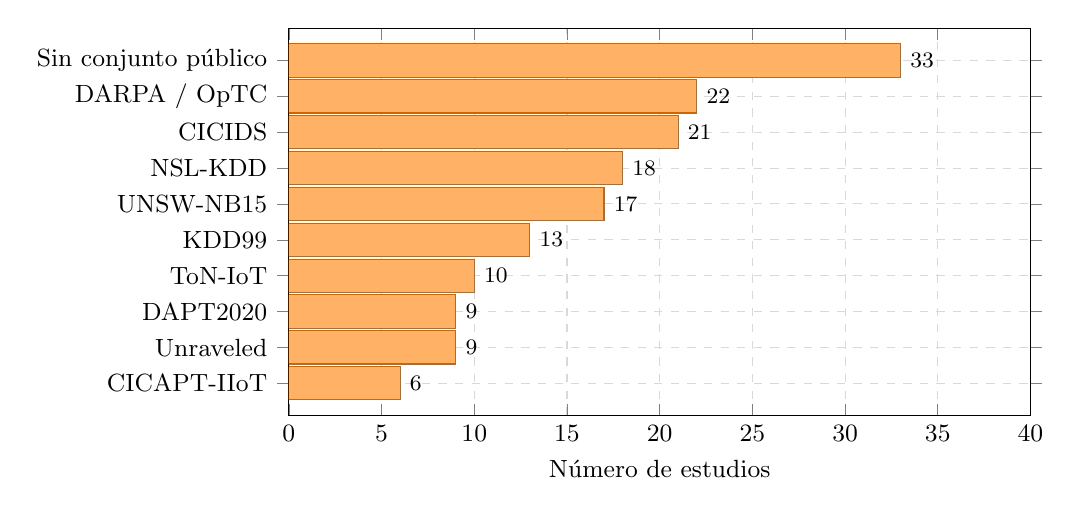
\begin{tikzpicture}
\begin{axis}[
    width=11cm, height=6.5cm,
    xbar, bar width=12pt,
    xmin=0, xmax=40,
    symbolic y coords={CICAPT-IIoT,Unraveled,DAPT2020,ToN-IoT,KDD99,UNSW-NB15,NSL-KDD,CICIDS,{DARPA / OpTC},{Sin conjunto público}},
    ytick=data,
    xlabel={Número de estudios},
    nodes near coords, nodes near coords style={font=\footnotesize},
    grid=major, grid style={dashed,gray!30},
    tick label style={font=\small}, label style={font=\small},
]
\addplot[fill=orange!60,draw=orange!80!black] coordinates {(6,CICAPT-IIoT)(9,Unraveled)(9,DAPT2020)(10,ToN-IoT)(13,KDD99)(17,UNSW-NB15)(18,NSL-KDD)(21,CICIDS)(22,{DARPA / OpTC})(33,{Sin conjunto público})};
\end{axis}
\end{tikzpicture}
\caption{Conjuntos de datos mencionados en los estudios del corpus. Fuente: Elaboración propia.}
\label{fig:datasets}
\end{figure}
\FloatBarrier

Entre los conjuntos con etiquetado por etapas de ataque, DAPT2020 \parencite{myneni2020dapt2020} y Unraveled \parencite{myneni2023unraveled} son los que presentan mayor correspondencia con los requerimientos de un modelo secuencial, dado que su estructura identifica explícitamente la fase de la campaña a la que corresponde cada registro. Ambos conjuntos han sido empleados conjuntamente en trabajos recientes de detección de APT \parencite{rivas_analysis_2025}. Los conjuntos de intrusiones de uso general, como NSL-KDD, CICIDS o UNSW-NB15, carecen de este etiquetado y presentan una separación entre tráfico legítimo y malicioso que no refleja la sofisticación de un adversario APT.

La literatura reciente documenta de forma explícita estas limitaciones. \textcite{mamun_limitations_2024} analizan sistemáticamente los conjuntos de datos disponibles para investigación en APT y concluyen que tienden a cubrir periodos breves, a subrepresentar las etapas intermedias de la campaña y a presentar distribuciones de clase que no reproducen las condiciones de operación reales. Esta constatación ha motivado la aparición de nuevos conjuntos orientados a corregir dichas carencias, entre ellos el benchmark propuesto por \textcite{liu_new_2022}, el conjunto CYSAS-S3 \parencite{choumanof_introducing_2022}, el conjunto de malware con atribución a grupos APT de \textcite{erfan_mazaheri_aptracker_2024} y, más recientemente, el conjunto cAPTure \parencite{puccetti_capture_2026}, orientado específicamente a evaluar la rapidez de detección. La persistencia de esta línea de trabajo confirma que la disponibilidad de datos representativos constituye un problema abierto en el área, y fundamenta la decisión de emplear dos conjuntos complementarios en el presente trabajo.

\section{Estrategias frente al desbalance de clases (RQ4)}

Treinta y seis estudios del corpus abordan explícitamente el problema del desbalance de clases en la detección de amenazas, cerca de la mitad del total. Las estrategias identificadas se concentran en técnicas de remuestreo, entre las que predomina el sobremuestreo sintético de la clase minoritaria \parencite{chawla2002smote}, junto con aproximaciones híbridas que combinan sobremuestreo y submuestreo. Estas técnicas operan sobre instancias tratadas como independientes entre sí, supuesto cuyas implicancias para un modelo secuencial se discuten en el Capítulo~\ref{cap:propuesta}.

No obstante, el hallazgo más significativo de esta dimensión no proviene de las estrategias empleadas, sino de las métricas utilizadas para evaluarlas. Como muestra la Figura~\ref{fig:metricas}, 35 estudios del corpus reportan \textit{accuracy}, mientras que solo 14 reportan F1-score, 8 precisión y 6 exhaustividad. Esta distribución resulta problemática: en escenarios con desbalance severo, donde la actividad maliciosa constituye una fracción mínima del tráfico total, la exactitud global puede alcanzar valores elevados aun cuando el modelo falle sistemáticamente en la clase minoritaria, que es precisamente la de interés.

\begin{figure}[h!]
\centering
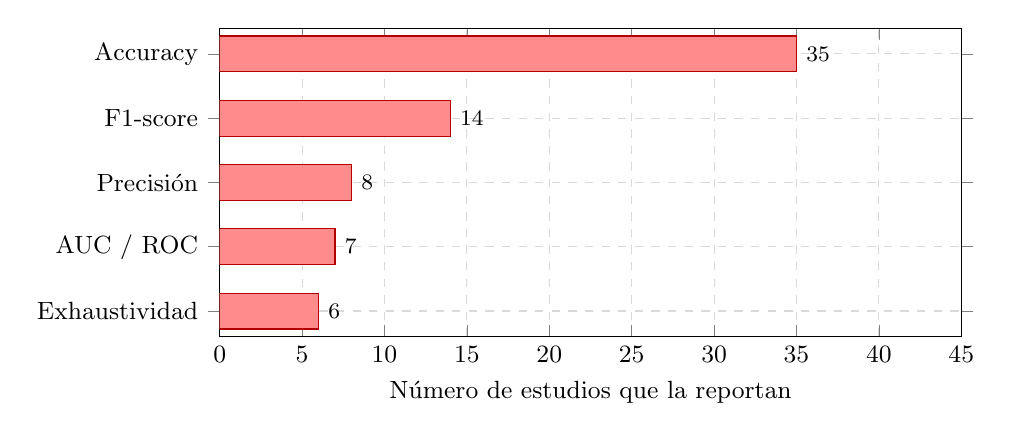
\begin{tikzpicture}
\begin{axis}[
    width=11cm, height=5.5cm,
    xbar, bar width=13pt,
    xmin=0, xmax=45,
    symbolic y coords={Exhaustividad,{AUC / ROC},Precisión,F1-score,Accuracy},
    ytick=data,
    xlabel={Número de estudios que la reportan},
    nodes near coords, nodes near coords style={font=\footnotesize},
    grid=major, grid style={dashed,gray!30},
    tick label style={font=\small}, label style={font=\small},
]
\addplot[fill=red!45,draw=red!70!black] coordinates {(6,Exhaustividad)(7,{AUC / ROC})(8,Precisión)(14,F1-score)(35,Accuracy)};
\end{axis}
\end{tikzpicture}
\caption{Métricas de evaluación reportadas en los estudios del corpus. Fuente: Elaboración propia.}
\label{fig:metricas}
\end{figure}
\FloatBarrier

En consecuencia, una proporción considerable de la literatura evalúa sus propuestas mediante una métrica que enmascara el problema que declara abordar, y son minoría los trabajos que reportan el desempeño de forma desagregada por clase o por etapa de ataque.

\section{Síntesis y brechas identificadas}

El análisis del corpus permite identificar cuatro brechas que fundamentan la propuesta de este trabajo.

\begin{itemize}
    \item En primer lugar, los modelos probabilísticos aplicados a la detección de APT operan mayoritariamente sobre alertas o indicadores previamente correlacionados, lo que introduce una dependencia respecto de una infraestructura de detección previa.
    \item En segundo lugar, si bien los Modelos Ocultos de Markov cuentan con precedentes consolidados en el dominio, su aplicación directa sobre tráfico de red etiquetado por etapas de ataque se encuentra escasamente explorada.
    \item En tercer lugar, no existe un conjunto de datos de referencia consolidado para la evaluación de propuestas en el área, y los conjuntos con etiquetado por etapas presentan una adopción limitada pese a ser los más adecuados para enfoques secuenciales.
    \item En cuarto lugar, y de manera transversal, la literatura evalúa predominantemente mediante métricas globales que no permiten observar el desempeño sobre la clase minoritaria, lo que impide determinar si las propuestas existentes mantienen su efectividad bajo las condiciones de desbalance que caracterizan a los escenarios reales.
\end{itemize}

Estas cuatro brechas configuran el espacio de oportunidad que aborda la propuesta descrita en el capítulo siguiente.
\chapter{Plan de Trabajo}
\label{cap:plan}

Esta sección presenta el plan de trabajo del proyecto. La planificación se organiza en dos etapas que abarcan dos semestres. La primera corresponde al Seminario de Título (segundo semestre 2026), que incluye la planificación de la investigación, el desarrollo del Estado del Arte y la propuesta preliminar. La segunda etapa corresponde al Proyecto de Título (primer semestre 2027), donde se desarrolla e implementa la propuesta de solución, se ejecutan los experimentos y se redacta el informe final.

\section{Carta Gantt}
La figura \ref{fig:gantt1} presenta el cronograma integrado del segundo semestre 2026. En el cual se inicia Seminario de Título, con foco en el desarrollo de la metodología, Estado del Arte y propuesta de solución a nivel de componentes y las características de este.

\begin{figure}[htbp]
    \centering
    \makebox[\textwidth][c]{%
        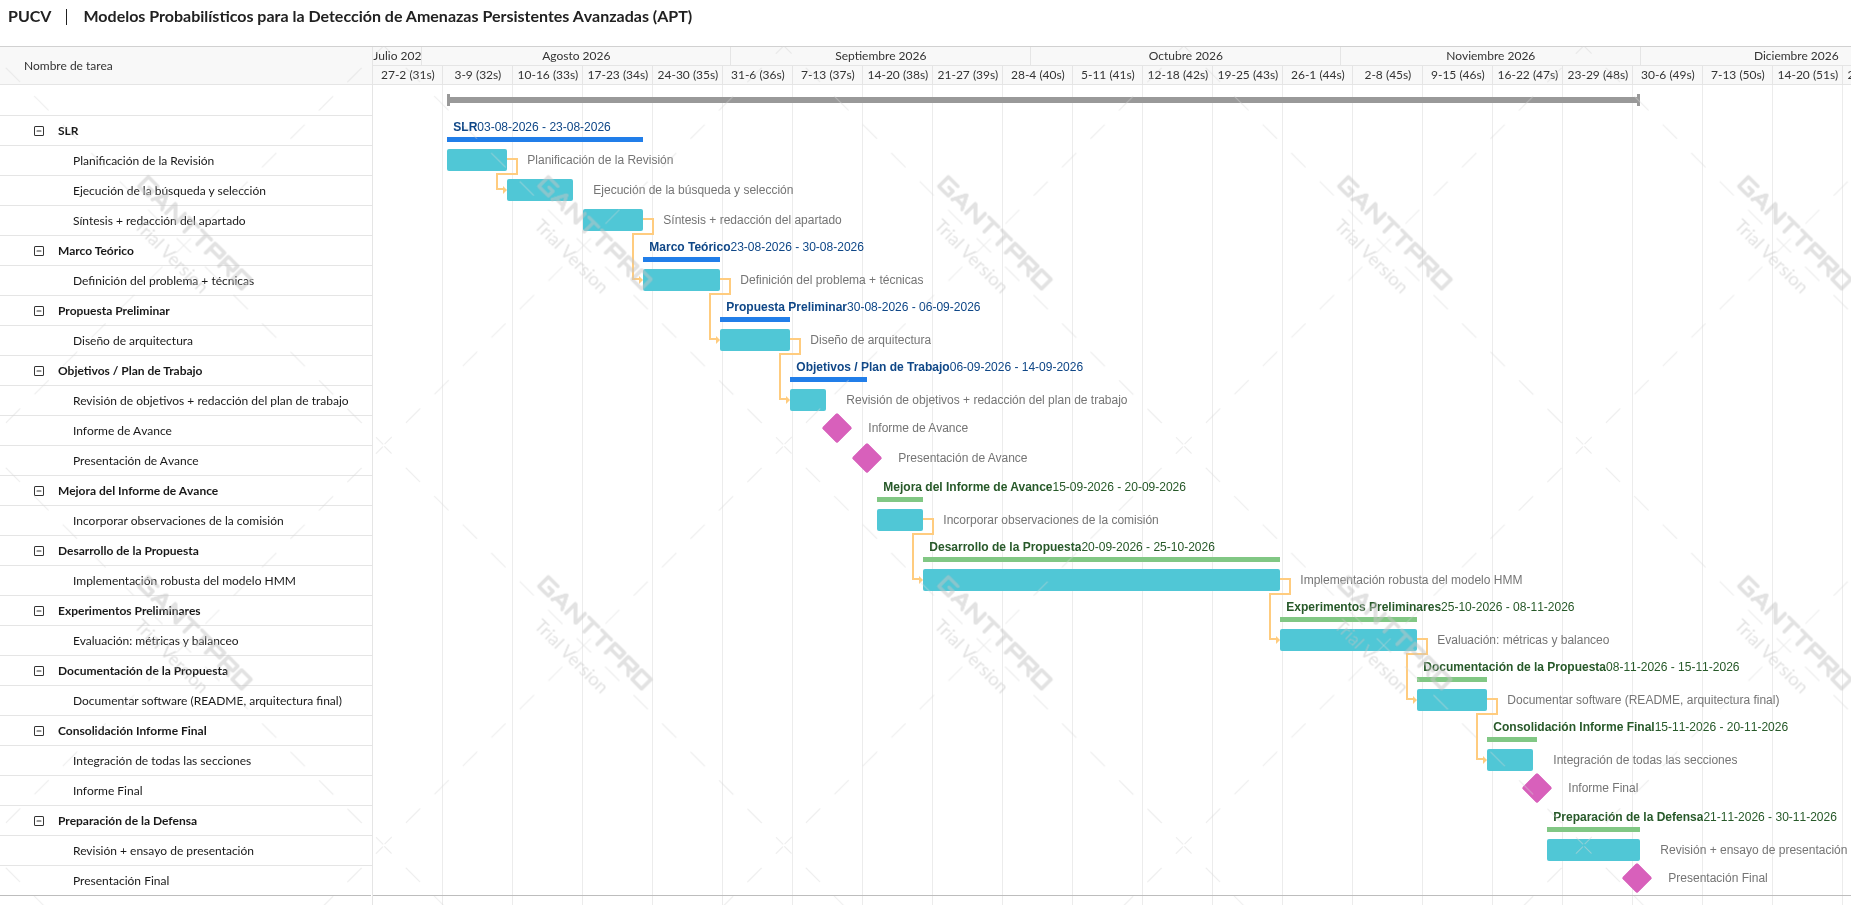
\includegraphics[width=0.95\paperwidth]{assets/CartaGantt1.png}%
    }
    \caption{Cronograma de actividades del Seminario de Título (agosto a noviembre de 2026). Fuente: Elaboración propia.}
    \label{fig:gantt1}
\end{figure}

\clearpage
\noindent
La Figura~\ref{fig:gantt2} presenta una planificación tentativa del primer semestre 2027, correspondiente a Proyecto de Título, con foco en el desarrollo e implementación completa de la propuesta de solución, las pruebas del sistema, la obtención de métricas de validación y la redacción del informe definitivo con los análisis de los resultados obtenidos. Dado que el calendario académico de dicho periodo aún no ha sido publicado, las fechas presentadas corresponden a estimaciones basadas en la duración habitual de un semestre y quedan sujetas a ajuste una vez que la Escuela fije las instancias formales de evaluación.

\vspace{0.5cm}

\begin{center}
    \makebox[\textwidth][c]{%
        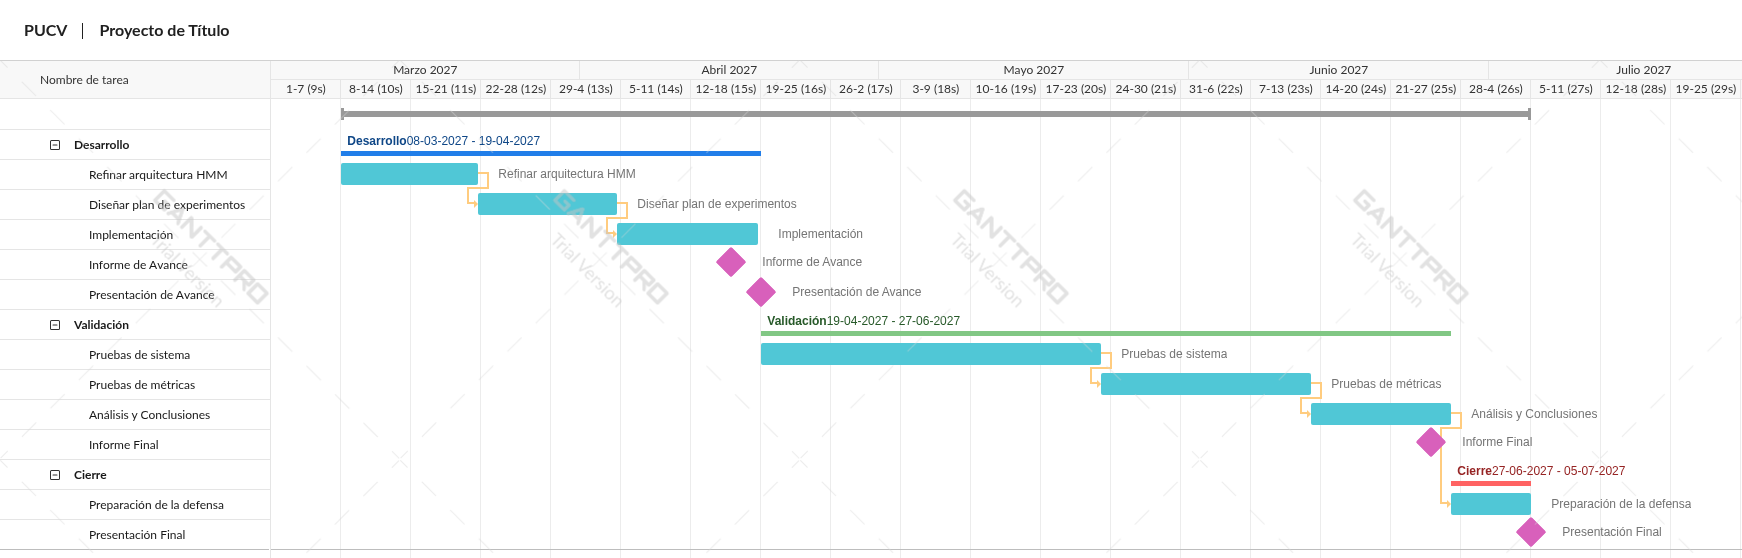
\includegraphics[width=0.95\paperwidth]{assets/CartaGantt2.png}%
    }
    \vspace{0.3cm}
    \captionof{figure}{Cronograma de actividades del Proyecto de Título (marzo a julio de 2027). Fuente: Elaboración propia.}
    \label{fig:gantt2}
\end{center}

\chapter{Propuesta de Solución}
\label{cap:propuesta}
Este capítulo presenta la propuesta de solución desarrollada a partir de los hallazgos de la revisión sistemática de la literatura. Las decisiones aquí expuestas constituyen la base de diseño conceptual y formal del artefacto, cuya codificación, calibración y validación experimental se desarrollarán en el Proyecto de Título conforme al plan de trabajo establecido.

\section{De las brechas identificadas a las decisiones de diseño}
Las decisiones arquitectónicas adoptadas responden directamente a las cuatro brechas identificadas en el Estado del Arte, garantizando una trazabilidad metodológica entre la evidencia secundaria y el diseño del artefacto. La Tabla \ref{tab:trazabilidad_brechas} resume esta correspondencia.

\begin{table}[h!]
\centering
\small
\renewcommand{\arraystretch}{1.25}
\begin{tabular}{|c|p{6.5cm}|p{7cm}|}
\hline
\textbf{RQ} & \textbf{Brecha identificada en la literatura} & \textbf{Decisión de diseño} \\ \hline
\textbf{RQ1} & Los modelos probabilísticos aplicados a APT operan mayoritariamente sobre alertas o grafos previamente correlacionados, generando dependencia de una infraestructura previa. & El modelo se diseña para operar directamente sobre registros de tráfico de red, suprimiendo la dependencia de subsistemas externos de correlación. \\ \hline
\textbf{RQ2} & Los estudios con HMM definen variables observables a partir de alertas de terceros; su modelación sobre tráfico estructurado por etapas está poco explorada. & Las variables observables se derivan de características estadísticas del flujo de red, y los estados ocultos se anclan a las fases de ataque etiquetadas en los conjuntos de datos (Sección~\ref{sec:correspondencia}). \\ \hline
\textbf{RQ3} & Ausencia de un benchmark consolidado y baja representatividad temporal en los conjuntos de datos comúnmente evaluados. & Se adopta una estrategia dual con DAPT2020 (comparabilidad histórica) y Unraveled (seis semanas de emulación organizacional realista). \\ \hline
\textbf{RQ4} & La mayoría de los estudios que reportan métricas utiliza \textit{Accuracy} global (35 de 77 estudios, frente a 14 que reportan $F_1$-score), lo que enmascara el desempeño sobre la clase minoritaria. & Evaluación con métricas desagregadas por etapa y métricas de detección temprana; tratamiento del desbalance que preserva la estructura temporal; comparación con modelos de referencia bajo las mismas condiciones. \\ \hline
\end{tabular}
\caption{Trazabilidad entre brechas de la revisión sistemática y decisiones de diseño.}
\label{tab:trazabilidad_brechas}
\end{table}

\section{Componentes de la propuesta}

\subsection{Entradas y preprocesamiento}
El sistema recibirá flujos de red provenientes de DAPT2020 y Unraveled. El preprocesamiento contempla:
\begin{enumerate}
    \item \textbf{Agregación temporal:} Los registros de flujo se agruparán por host en ventanas de tiempo $\Delta t$, ordenadas según su instante de inicio. Cada secuencia corresponde a la actividad de un host a lo largo del periodo registrado.
    \item \textbf{Vector de observaciones:} Se seleccionará un conjunto acotado de atributos representativos (tasa de bytes, duración del flujo, distribución de puertos y flags TCP), los cuales serán discretizados mediante cuantización por intervalos para conformar el alfabeto de símbolos observables $V = \{v_1, \dots, v_M\}$. Los límites de los intervalos se calcularán solo con la partición de entrenamiento.
    \item \textbf{Etiquetado de ventanas:} Se construirá una tabla de correspondencia entre las etiquetas de etapa de cada conjunto de datos y los cinco estados del modelo. Una ventana se etiquetará como benigna si no contiene flujos maliciosos y, en caso contrario, con la etapa de mayor avance presente entre sus flujos. La sensibilidad de esta regla y del tamaño de $\Delta t$ se evaluará experimentalmente.
\end{enumerate}

\subsection{Definición formal del modelo generativo}
El núcleo de procesamiento se modela formalmente como una tupla $\lambda = (A, B, \pi)$:
\begin{itemize}
    \item \textbf{Estados Ocultos ($S$):} Representan las etapas no visibles del ataque: $S = \{s_{\text{benigno}}, s_{\text{reconocimiento}}, \newline s_{\text{foothold}}, s_{\text{lateral}}, s_{\text{exfiltracion}}\}$.
    \item \textbf{Matriz de Transición ($A$):} Matriz estocástica $N \times N$ que modela la probabilidad de evolución secuencial del adversario entre etapas.
    \item \textbf{Matriz de Emisión ($B$):} Matriz $N \times M$ que define la probabilidad de registrar un determinado patrón de tráfico $v_k$ condicionada al estado activo $s_j$.
    \item \textbf{Distribución Inicial ($\pi$):} Vector de probabilidades de inicio del proceso.
\end{itemize}
Los parámetros se estimarán de forma supervisada a partir de las secuencias etiquetadas y se refinarán con Baum-Welch bajo restricciones, según se detalla en la Sección~\ref{sec:correspondencia}. La inferencia en línea se realizará mediante la probabilidad filtrada, y la reconstrucción retrospectiva de la secuencia completa de etapas mediante el algoritmo de Viterbi.

\subsection{Salidas esperadas}
Ante una secuencia de observaciones $O = (O_1, \dots, O_T)$, el modelo reportará:
\begin{itemize}
    \item En cada instante $t$, la etapa más probable según la probabilidad filtrada $P(q_t \mid O_1, \dots, O_t, \lambda)$, junto con su nivel de confianza y la probabilidad de transición hacia la siguiente fase de la campaña, estimada a partir de $A$.
    \item Una alerta cuando la probabilidad acumulada de los estados de ataque supere un umbral $\tau$ calibrado en la partición de validación.
    \item De forma retrospectiva, la secuencia óptima de estados $Q^* = (q_1^*, \dots, q_T^*)$ obtenida con Viterbi, que reconstruye la progresión completa del ataque para su análisis forense.
\end{itemize}

\section{Correspondencia entre estados ocultos y etapas de ataque}
\label{sec:correspondencia}
Como se expuso en el Marco Teórico, Baum-Welch sin supervisión no garantiza que los estados aprendidos correspondan a Reconocimiento, Foothold, Movimiento lateral y Exfiltración: el algoritmo converge a un máximo local y la verosimilitud es invariante ante permutaciones de los estados. Para asegurar esta correspondencia se adopta una estrategia en tres niveles, que aprovecha que DAPT2020 y Unraveled proveen etiquetas de etapa.

\begin{enumerate}
    \item \textbf{Anclaje por supervisión.} Los parámetros $\hat{A}$, $\hat{B}$ y $\hat{\pi}$ se estiman mediante conteo de frecuencias sobre las secuencias etiquetadas de entrenamiento (estimación de máxima verosimilitud), con suavizado de Laplace. Cada estado queda así vinculado a su etapa por construcción, y la fila de $B$ asociada a, por ejemplo, el movimiento lateral se calcula exclusivamente con ventanas etiquetadas como tal.
    \item \textbf{Refinamiento restringido.} El algoritmo de Baum-Welch se utiliza solo como refinamiento, inicializado con la estimación supervisada y no con valores aleatorios. Las transiciones que no se observan en el entrenamiento y que son inconsistentes con la cadena de ataque se fijan en cero, propiedad que la reestimación conserva. La estructura no se restringe a un orden estrictamente lineal, ya que un atacante puede volver a etapas previas, por ejemplo, reconocimiento interno tras el movimiento lateral. Para limitar la deriva semántica de los estados, el número de iteraciones se controla con la verosimilitud sobre la partición de validación.
    \item \textbf{Verificación posterior.} Tras el entrenamiento, se verificará la correspondencia comparando la etapa inferida con la etiqueta real en la partición de validación mediante una matriz de confusión por estado. Si la exactitud de algún estado respecto de su etiqueta se degrada frente a la estimación supervisada, el refinamiento se descarta para ese conjunto de datos. Adicionalmente, se comparará cada fila de $B$ con el perfil empírico de tráfico de su etapa.
\end{enumerate}

Como experimento de control, se entrenará también un HMM con Baum-Welch desde una inicialización aleatoria y sin supervisión. Sus estados se asignarán a las etapas mediante el emparejamiento óptimo con las etiquetas (algoritmo húngaro sobre la matriz de coincidencias). Este control permitirá cuantificar cuánto de la correspondencia se pierde cuando los estados no se anclan a las etapas, y justificar empíricamente la estrategia adoptada.

\section{Tratamiento del desbalance de clases}
\label{sec:desbalance}
Dado que SMOTE genera instancias sin posición temporal y no está definido sobre símbolos discretos, no se aplicará sobre las secuencias del HMM. El tratamiento del desbalance se diferencia según el tipo de modelo:

\begin{itemize}
    \item \textbf{Para el HMM}, se contrastarán tres condiciones que preservan la estructura temporal:
    \begin{enumerate}
        \item \textit{Datos originales con suavizado}: estimación supervisada sin remuestreo, con suavizado de Laplace sobre $A$, $B$ y $\pi$.
        \item \textit{Calibración del umbral de decisión}: el umbral $\tau$ sobre la probabilidad filtrada de los estados de ataque se ajusta en validación para una tasa objetivo de falsas alarmas, en lugar de asignar la etapa de mayor probabilidad.
        \item \textit{Remuestreo a nivel de secuencia}: en la partición de entrenamiento se replican secuencias completas que contienen actividad de ataque y se submuestrean tramos benignos alejados de dicha actividad, de modo que el orden interno de cada secuencia no se altera.
    \end{enumerate}
    \item \textbf{Para los modelos de referencia}, que tratan cada ventana como independiente, se contrastarán los datos originales, la ponderación de clases y SMOTE.
\end{itemize}

En todos los casos, el remuestreo se aplicará únicamente sobre la partición de entrenamiento, después de particionar los datos, y la evaluación se realizará siempre sobre la distribución original de clases.

\section{Métricas de evaluación}

\subsection{Desempeño por etapa}
Para cada etapa de ataque se reportarán la precisión, la exhaustividad y el $F_1$-score, junto con su promedio macro y la matriz de confusión entre etapas. Se descarta la exactitud global como métrica principal, por las razones expuestas en el Estado del Arte.

\subsection{Detección temprana}
Dado que el objetivo general del proyecto es la identificación temprana de la progresión de una APT, no basta con medir si una ventana se clasifica correctamente: es necesario medir \textit{cuándo} se detecta el ataque. Estas métricas se calculan con la inferencia en línea, es decir, utilizando en cada instante solo la evidencia disponible hasta ese momento.

Sea $\mathcal{C}$ el conjunto de secuencias atacadas, es decir, las secuencias de host que contienen al menos una ventana maliciosa. Para cada $c \in \mathcal{C}$, sea $t_0^c$ el inicio de la primera ventana maliciosa, $t_{\text{fin}}^c$ el final de la última y $t_{\text{exf}}^c$ el inicio de la etapa de exfiltración. El modelo emite una alerta en el instante $t$ cuando
\begin{equation}
P\big(q_t \in S_{\text{ataque}} \mid O_1, \dots, O_t, \lambda\big) \geq \tau, \qquad S_{\text{ataque}} = S \setminus \{s_{\text{benigno}}\}
\end{equation}
y se denota $t_d^c$ el primer instante de alerta con $t_d^c \geq t_0^c$. Las alertas anteriores a $t_0^c$ se contabilizan como falsas alarmas. A partir de estas definiciones se reportarán:

\begin{itemize}
    \item \textbf{Tiempo hasta la detección:} $\mathrm{TTD}_c = t_d^c - t_0^c$, resumido mediante su mediana y percentiles sobre $\mathcal{C}$.
    \item \textbf{Precocidad normalizada:} $\mathrm{E}_c = (t_d^c - t_0^c) / (t_{\text{fin}}^c - t_0^c) \in [0, 1]$, que expresa la fracción de la campaña transcurrida al momento de la detección y permite comparar campañas de distinta duración. Las campañas no detectadas se reportan por separado.
    \item \textbf{Etapa de primera detección:} la etapa real en el instante $t_d^c$, cuya distribución indica si los ataques se detectan durante el reconocimiento o solo cuando ya se encuentran avanzados.
    \item \textbf{Tasa de detección previa a la exfiltración:} proporción de secuencias atacadas en que $t_d^c < t_{\text{exf}}^c$, es decir, detectadas antes de que se materialice el daño principal.
    \item \textbf{Retardo por etapa:} para cada etapa $e$, el tiempo entre su inicio y la primera ventana en que el modelo la identifica correctamente.
\end{itemize}

Una detección temprana solo es útil si no se obtiene a costa de un exceso de alertas, ya que un detector que alerta en todas las ventanas alcanzaría un tiempo de detección nulo. Por ello, las métricas anteriores se reportarán junto con la tasa de falsas alarmas en los periodos benignos y se presentarán como una curva de compromiso entre el tiempo de detección y la tasa de falsos positivos al variar $\tau$, siguiendo la metodología de evaluación propuesta para el conjunto cAPTure, que relaciona ambas métricas como criterios prácticos de despliegue \parencite{puccetti_capture_2026}.

\subsection{Comparación con modelos de referencia}
\label{sec:baseline}
La comparación con resultados publicados no es suficiente para validar la propuesta, ya que los estudios difieren en el preprocesamiento, la partición de los datos y las métricas reportadas. Por ejemplo, \textcite{rivas_analysis_2025} evalúan Random Forest, árboles de decisión y XGBoost sobre DAPT2020 y Unraveled reportando exactitud, precisión, exhaustividad y $F_1$-score, pero con un preprocesamiento y una partición propios, por lo que sus resultados servirán solo como referencia contextual. Por ello se implementarán dos modelos de referencia, Random Forest \parencite{breiman2001random} y XGBoost \parencite{chen2016xgboost}, bajo las mismas condiciones que el HMM:

\begin{itemize}
    \item \textbf{Mismos datos y misma partición.} Los datos se particionarán en entrenamiento, validación y prueba agrupando por secuencia, de modo que ninguna secuencia quede dividida entre particiones, y respetando el orden cronológico cuando la estructura del conjunto lo permita. Se evita la partición aleatoria por ventana, ya que ventanas contiguas son casi idénticas y su separación entre entrenamiento y prueba sobreestimaría el desempeño.
    \item \textbf{Mismas ventanas, atributos y etiquetas.} Los modelos de referencia utilizarán las mismas ventanas $\Delta t$, los mismos atributos y la misma correspondencia de cinco etapas. Se evaluarán con los atributos continuos, su representación natural, y con los mismos símbolos discretos del HMM, para aislar el efecto de la discretización.
    \item \textbf{Variante con contexto temporal.} Se incluirá una variante de cada modelo de referencia que incorpora los atributos de las $k$ ventanas previas. Así, una eventual ventaja del HMM podrá atribuirse al modelado de la progresión entre etapas y no solo a disponer de información del pasado.
    \item \textbf{Mismas métricas.} Se reportarán las métricas por etapa y las de detección temprana. Para los modelos de referencia, la alerta se emite cuando la probabilidad estimada de una clase de ataque supera el umbral $\tau$, calibrado con el mismo criterio de falsas alarmas.
    \item \textbf{Mismo procedimiento de ajuste.} Los hiperparámetros de todos los modelos se ajustarán únicamente con la partición de validación.
\end{itemize}

\section{Diseño experimental}
La Tabla~\ref{tab:experimentos} resume las configuraciones que se evaluarán. Cada una se ejecutará sobre DAPT2020, para la comparación con la literatura, y sobre Unraveled, para evaluar la estabilidad del modelo en trazas longitudinales de seis semanas con desbalance severo.

\begin{table}[h!]
\centering
\small
\renewcommand{\arraystretch}{1.25}
\begin{tabularx}{\textwidth}{|c|p{3.4cm}|X|X|}
\hline
\textbf{ID} & \textbf{Modelo} & \textbf{Estimación} & \textbf{Tratamiento del desbalance} \\ \hline
H1 & HMM & Supervisada (conteo de frecuencias) & Original con suavizado; umbral calibrado; remuestreo por secuencia \\ \hline
H2 & HMM & Supervisada + Baum-Welch restringido & Igual que H1 \\ \hline
H0 & HMM (control) & Baum-Welch no supervisado, inicialización aleatoria & Original; se mide la correspondencia entre estados y etapas \\ \hline
B1 & Random Forest & Supervisada, con y sin contexto temporal & Original; ponderación de clases; SMOTE en entrenamiento \\ \hline
B2 & XGBoost & Supervisada, con y sin contexto temporal & Igual que B1 \\ \hline
\end{tabularx}
\caption{Configuraciones del diseño experimental.}
\label{tab:experimentos}
\end{table}

El diseño permite contrastar dos hipótesis de trabajo. La primera es que, a igual tasa de falsas alarmas, el HMM detecta las campañas antes y con mayor frecuencia previo a la exfiltración que los modelos de referencia, por modelar la progresión entre etapas. La segunda es que los modelos de referencia pueden alcanzar un $F_1$-score por ventana comparable o superior. Si ambas se confirman, el aporte del HMM radicaría en la detección temprana y la interpretabilidad de la progresión, más que en la clasificación aislada de ventanas. Los resultados se analizarán por conjunto de datos, por etapa y por condición de desbalance.

\chapter{Experimentos y Análisis Preliminares}
\label{cap:experimentos}
Este capítulo presenta una primera implementación del diseño descrito en el Capítulo~\ref{cap:propuesta} y los resultados de su ejecución sobre DAPT2020 y Unraveled. Su propósito es verificar que la propuesta es factible de punta a punta y detectar con anticipación los aspectos del diseño que requieren ajuste antes de su validación definitiva. Los resultados son preliminares: provienen de una única partición de los datos, de un número reducido de campañas atacadas y de una configuración que aún no ha sido congelada, por lo que no constituyen la validación experimental del modelo.

\section{Implementación del prototipo}
\label{sec:prototipo}
El prototipo se implementó en Python 3.13 como un paquete con un módulo por cada componente de la propuesta: carga y limpieza de los conjuntos de datos, construcción de ventanas por host, partición de los datos, discretización de las observables, estimación e inferencia del HMM, modelos de referencia, métricas de evaluación y orquestación de los experimentos. La estimación supervisada por conteo, la inferencia filtrada y el algoritmo de Viterbi se implementaron directamente con NumPy, mientras que el refinamiento con Baum-Welch restringido y el control no supervisado se apoyan en la biblioteca hmmlearn. Los modelos de referencia utilizan scikit-learn, XGBoost e imbalanced-learn para SMOTE. El código del modelo probabilístico se presenta en el Anexo~\ref{anx:modelo}.

La corrección de los componentes se verifica con 44 pruebas automatizadas. Entre ellas, el filtrado y el algoritmo de Viterbi se contrastan con una enumeración exhaustiva de las secuencias de estados en un modelo pequeño, se comprueba que Baum-Welch conserva los ceros estructurales de la matriz de transición, que el emparejamiento mediante el algoritmo húngaro recupera una permutación conocida de los estados y que los límites de la discretización se calculan solo con la partición de entrenamiento. Cada ejecución guarda los parámetros con que fue realizada, y las semillas aleatorias son fijas, de modo que los resultados de este capítulo pueden reproducirse.

Los experimentos se ejecutaron en un computador personal, y las configuraciones de sensibilidad del HMM (Sección~\ref{sec:res_sensibilidad}) se ejecutaron además en un servidor de la universidad, para verificar que los resultados no dependen del equipo. Las 35 configuraciones ejecutadas en ambos equipos produjeron métricas idénticas, pese a las diferencias de procesador y de versión de Python. La Tabla~\ref{tab:entorno} resume las características de ambos equipos. El prototipo utiliza solo el procesador, por lo que la tarjeta gráfica del servidor no interviene en los cálculos. En el computador personal, las 31 configuraciones de DAPT2020 tomaron alrededor de un minuto. En Unraveled, las siete configuraciones del HMM tomaron cerca de ocho minutos y las 24 de referencia cerca de 25, la mayor parte en las variantes con contexto temporal.

\begin{table}[h!]
\centering
\small
\renewcommand{\arraystretch}{1.25}
\begin{tabularx}{\textwidth}{|>{\raggedright\arraybackslash}p{3cm}|>{\raggedright\arraybackslash}X|>{\raggedright\arraybackslash}X|}
\hline
\textbf{Característica} & \textbf{Computador personal} & \textbf{Servidor de la universidad} \\ \hline
Procesador & AMD Ryzen 5 5600G (6 núcleos, 12 hilos) & Intel Core i9-10900K a 3,70 GHz (10 núcleos, 20 hilos) \\ \hline
Memoria RAM & 16 GB & 64 GB a 2.400 MHz \\ \hline
Tarjeta gráfica & Integrada (no utilizada) & NVIDIA GeForce RTX 3060 de 12 GB (no utilizada) \\ \hline
Almacenamiento & SSD & SSD de 932 GB \\ \hline
Sistema operativo & Windows 11 Pro de 64 bits & Windows de 64 bits \\ \hline
Python & 3.13 & 3.12 \\ \hline
\end{tabularx}
\caption{Características de los equipos de ejecución. Fuente: Elaboración propia.}
\label{tab:entorno}
\end{table}
\FloatBarrier

\section{Configuración experimental}
\label{sec:config_experimental}
Los aspectos que el Capítulo~\ref{cap:propuesta} dejó abiertos se fijaron como se describe a continuación.

\begin{itemize}
    \item \textbf{Limpieza.} En DAPT2020, uno de los archivos de flujos no incluye fila de encabezado y contiene la mayor parte del movimiento lateral, por lo que se lee con el encabezado de los demás archivos. En Unraveled, 13.169 filas tenían comas dentro de un campo de texto, lo que desplazaba sus columnas. Esas filas se repararon en lugar de excluirse, con lo que el conjunto queda en 6.877.157 flujos. La diferencia con el recuento de la Tabla~\ref{tab:datasets_eval} corresponde exactamente a esas filas.
    \item \textbf{Secuencias.} Cada secuencia corresponde a la actividad de un host interno de la organización, y cada flujo se asigna a su extremo interno. En Unraveled se consideran los 46 hosts internos con más de 1.000 flujos, y en DAPT2020 los 6 hosts internos con más de 100 flujos.
    \item \textbf{Ventanas y observables.} Las ventanas tienen una duración $\Delta t$ de cinco minutos, sin solapamiento. En cada una se calculan cuatro atributos por host: el volumen de bytes enviados, la mediana de la duración de los flujos, el número de puertos de destino distintos y la proporción de conexiones fallidas. Cada atributo se discretiza en tres niveles con cortes en los percentiles 50 y 95 de las ventanas de entrenamiento, y el símbolo observable es la combinación de los cuatro niveles. Con un símbolo adicional para las ventanas sin actividad, el alfabeto tiene $M = 82$ símbolos.
    \item \textbf{Etiquetas.} Cada ventana recibe la etapa más avanzada presente entre sus flujos, y el encubrimiento de Unraveled se asigna a la exfiltración.
    \item \textbf{Partición.} En Unraveled, la partición es cronológica: el entrenamiento comprende del 26 de mayo al 26 de junio de 2021, la validación del 27 al 29 de junio y la prueba del 30 de junio al 6 de julio. En DAPT2020, como cada etapa ocurre en un día distinto, cada captura diaria se divide en orden cronológico en un 60~\% para entrenamiento, un 20~\% para validación y un 20~\% para prueba.
    \item \textbf{Episodios de ataque.} Para las métricas de detección temprana, un episodio es un tramo de ventanas maliciosas de un mismo host separado de otros por al menos seis horas sin actividad maliciosa.
    \item \textbf{Ajuste.} El suavizado aditivo de la matriz de emisión se elige en validación entre los valores 0,01, 0,1 y 1, y en la configuración base resultó elegido el valor 0,01 en ambos conjuntos. El umbral $\tau$ se calibra en validación para una tasa de falsas alarmas de 1~\% de las ventanas benignas en DAPT2020 y de 0,1~\% en Unraveled. En DAPT2020 se usa un valor mayor porque su partición de validación tiene menos de 600 ventanas benignas.
\end{itemize}

La Tabla~\ref{tab:ventanas_particion} resume las ventanas resultantes por etapa y partición. En Unraveled, el reconocimiento de entrenamiento proviene solo del grupo APT y el de prueba solo del atacante aficionado, por lo que esa etapa mide la generalización entre atacantes. En DAPT2020, la exfiltración dispone de solo cinco ventanas de entrenamiento y cuatro de prueba.

\begin{table}[h!]
\centering
\small
\renewcommand{\arraystretch}{1.25}
\begin{tabular}{|l|r|r|r|r|r|r|}
\hline
 & \multicolumn{3}{c|}{\textbf{DAPT2020}} & \multicolumn{3}{c|}{\textbf{Unraveled}} \\ \hline
\textbf{Etapa} & \textbf{Entren.} & \textbf{Valid.} & \textbf{Prueba} & \textbf{Entren.} & \textbf{Valid.} & \textbf{Prueba} \\ \hline
Benigno & 1.894 & 589 & 562 & 387.998 & 32.879 & 75.044 \\ \hline
Reconocimiento & 18 & 3 & 7 & 675 & 6 & 106 \\ \hline
\textit{Foothold} & 33 & 11 & 9 & 1.314 & 750 & 709 \\ \hline
Movimiento lateral & 36 & 26 & 30 & 1.446 & 651 & 478 \\ \hline
Exfiltración & 5 & 1 & 4 & 349 & 720 & 1.035 \\ \hline
Episodios de ataque & & & 8 & & & 15 \\ \hline
\end{tabular}
\caption[Ventanas de cinco minutos por etapa y partición.]{Ventanas de cinco minutos por etapa y partición, y episodios de ataque en la partición de prueba. Fuente: Elaboración propia.}
\label{tab:ventanas_particion}
\end{table}
\FloatBarrier

Se ejecutaron las 31 configuraciones derivadas de la Tabla~\ref{tab:experimentos} en cada conjunto de datos. Las siete del HMM corresponden a H1 y H2 bajo las tres condiciones de desbalance más el control H0. Las 24 de referencia combinan los dos modelos, los atributos continuos o discretizados, la presencia o ausencia de contexto temporal y los tres tratamientos del desbalance. En la variante con contexto, el número de ventanas previas $k \in \{1, 3, 6\}$ y la profundidad de los árboles se eligieron en validación. Las Tablas~\ref{tab:res_unraveled} y~\ref{tab:res_dapt} presentan las configuraciones del HMM y, de los modelos de referencia, las que usan atributos continuos y datos originales, con y sin contexto. Se reporta siempre el mismo subconjunto para no seleccionar las configuraciones según su resultado en prueba.

\subsection{Alcance de los experimentos preliminares}
\label{sec:alcance_experimentos}
Los experimentos de este capítulo se acotaron deliberadamente, por las razones que se exponen a continuación.

\begin{itemize}
    \item \textbf{Propósito de los experimentos.} Estos experimentos buscan verificar que cada componente funciona de punta a punta y que todas las métricas pueden calcularse, no seleccionar todavía la mejor configuración. Por ello, se ejecutó una sola vez la matriz completa de la Tabla~\ref{tab:experimentos} en ambos conjuntos de datos.
    \item \textbf{Un factor a la vez.} En las sensibilidades se modificó un solo aspecto respecto de la configuración base, para que cualquier cambio en los resultados pueda atribuirse a ese aspecto. Combinar todas las alternativas evaluadas, es decir, tres tamaños de ventana, tres discretizaciones y dos tratamientos del encubrimiento, requeriría 18 variantes en lugar de 6. Con solo siete episodios atacados en la partición de validación, comparar tantas variantes aumentaría el riesgo de elegir una configuración que solo funciona bien por azar en ese periodo. Las combinaciones se evaluarán una vez identificados los factores que mejoran por separado, que según los resultados de la Sección~\ref{sec:res_sensibilidad} son la ventana de un minuto y la discretización por terciles.
    \item \textbf{Sensibilidades solo sobre el HMM.} Las sensibilidades tienen por objeto elegir el preprocesamiento del HMM. Los modelos de referencia se ejecutarán una sola vez con la configuración elegida, para compararlos con el HMM bajo las mismas condiciones. Además, son los que concentran la mayor parte del tiempo de ejecución, y la ventana de un minuto multiplica por cinco el número de ventanas.
    \item \textbf{Uso de la partición de prueba.} Cada configuración evaluada en prueba aumenta el riesgo de ajustar el diseño a ese periodo. Por ello, la matriz completa se evaluó en prueba una sola vez, con fines exploratorios, y las sensibilidades se evaluaron en validación.
\end{itemize}

Quedan pendientes, conforme al plan de trabajo, la combinación de los factores que mejoraron por separado, la sensibilidad de la regla de etiquetado de las ventanas, la validación cruzada agrupada por día y el análisis separado por grupo atacante.

\section{Resultados preliminares}
\label{sec:resultados_preliminares}

\subsection{Desempeño por etapa}
La Tabla~\ref{tab:res_unraveled} muestra los resultados en la partición de prueba de Unraveled. El HMM supervisado identifica el \textit{foothold} con un $F_1$-score de 0,740 y el movimiento lateral con una exhaustividad de 0,868, pero con una precisión de solo 0,096 en esta última etapa, ya que asigna 3.814 ventanas benignas al movimiento lateral. Las 12 configuraciones de referencia con atributos continuos superan al HMM en ambas etapas, con $F_1$-score entre 0,841 y 0,964 en el \textit{foothold} y entre 0,457 y 0,781 en el movimiento lateral. Considerando las 24 configuraciones de referencia, el $F_1$-score macro sobre las etapas de ataque varía entre 0,053 y 0,433, frente a 0,228 del HMM supervisado.

\begin{table}[h!]
\centering
\small
\renewcommand{\arraystretch}{1.25}
\begin{tabular}{|l|c|c|c|c|c|c|c|c|}
\hline
\textbf{Configuración} & \textbf{Rec.} & \textbf{Foot.} & \textbf{Lat.} & \textbf{Exf.} & \textbf{Macro} & \textbf{FPR} & \textbf{Detec.} & \textbf{TTD} \\ \hline
H1 original & 0,000 & 0,740 & 0,173 & 0,000 & 0,228 & 0,75~\% & 4/15 & 55 \\ \hline
H1 umbral & 0,000 & 0,786 & 0,000 & 0,000 & 0,197 & 0,75~\% & 4/15 & 55 \\ \hline
H1 remuestreo & 0,000 & 0,750 & 0,171 & 0,003 & 0,231 & 0,18~\% & 5/15 & 65 \\ \hline
H0 (control) & 0,000 & 0,000 & 0,060 & 0,084 & 0,036 & 1,40~\% & 9/15 & 45 \\ \hline
RF sin contexto & 0,000 & 0,841 & 0,457 & 0,000 & 0,325 & 1,01~\% & 11/15 & 10 \\ \hline
RF con contexto & 0,000 & 0,876 & 0,494 & 0,000 & 0,343 & 1,53~\% & 10/15 & 15 \\ \hline
XGBoost sin contexto & 0,000 & 0,864 & 0,474 & 0,000 & 0,334 & 0,88~\% & 11/15 & 5 \\ \hline
XGBoost con contexto & 0,000 & 0,964 & 0,567 & 0,002 & 0,383 & 1,25~\% & 12/15 & 10 \\ \hline
\end{tabular}
\caption[Resultados preliminares en la partición de prueba de Unraveled.]{Resultados preliminares en la partición de prueba de Unraveled. Rec., Foot., Lat. y Exf.: $F_1$-score de cada etapa. Macro: promedio de los cuatro. FPR: proporción de ventanas benignas con alerta. Detec.: episodios detectados. TTD: mediana del tiempo hasta la detección en minutos, sobre los episodios detectados. H2 no se muestra porque coincide con H1 (Sección~\ref{sec:res_correspondencia}). Fuente: Elaboración propia.}
\label{tab:res_unraveled}
\end{table}
\FloatBarrier

Dos etapas no son identificadas por ningún modelo en Unraveled. En el reconocimiento, ninguna de las 31 configuraciones supera un $F_1$-score de 0,001. Como el reconocimiento de entrenamiento proviene del grupo APT y el de prueba del atacante aficionado, este resultado indica que los patrones aprendidos de un atacante no se trasladan al otro con las observables actuales. En la exfiltración, el HMM asigna 967 de las 1.035 ventanas de prueba al estado benigno, y ninguna configuración de referencia supera un $F_1$-score de 0,031 en esa etapa. Con los cuatro atributos definidos, las ventanas de exfiltración de prueba no se distinguen del tráfico benigno, aunque en la partición de validación esa etapa sí se identifica (Sección~\ref{sec:res_sensibilidad}).

La Tabla~\ref{tab:res_dapt} muestra los resultados en DAPT2020. Todos los modelos obtienen valores bajos, con un $F_1$-score macro entre 0,012 y 0,188 en las configuraciones de referencia y de 0,099 en el HMM supervisado. El HMM no identifica el movimiento lateral ni la exfiltración. En esta última etapa, que cuenta con cuatro ventanas de prueba, solo cuatro configuraciones de referencia, todas con atributos discretizados y ponderación de clases, obtienen un $F_1$-score positivo, con un máximo de 0,148. Con tan pocas ventanas por etapa, una sola ventana modifica de forma apreciable estas métricas, por lo que los resultados de DAPT2020 se interpretan solo como comparativos.

\begin{table}[h!]
\centering
\small
\renewcommand{\arraystretch}{1.25}
\begin{tabular}{|l|c|c|c|c|c|c|c|c|}
\hline
\textbf{Configuración} & \textbf{Rec.} & \textbf{Foot.} & \textbf{Lat.} & \textbf{Exf.} & \textbf{Macro} & \textbf{FPR} & \textbf{Detec.} & \textbf{TTD} \\ \hline
H1 original & 0,261 & 0,136 & 0,000 & 0,000 & 0,099 & 1,60~\% & 3/8 & 5 \\ \hline
H1 umbral & 0,125 & 0,154 & 0,000 & 0,000 & 0,070 & 1,60~\% & 3/8 & 5 \\ \hline
H1 remuestreo & 0,240 & 0,140 & 0,000 & 0,000 & 0,095 & 1,60~\% & 2/8 & 42,5 \\ \hline
H0 (control) & 0,167 & 0,093 & 0,000 & 0,000 & 0,065 & 0,00~\% & 0/8 & n. a. \\ \hline
RF sin contexto & 0,375 & 0,176 & 0,000 & 0,000 & 0,138 & 1,96~\% & 3/8 & 10 \\ \hline
RF con contexto & 0,154 & 0,087 & 0,065 & 0,000 & 0,076 & 1,78~\% & 3/8 & 55 \\ \hline
XGBoost sin contexto & 0,375 & 0,138 & 0,000 & 0,000 & 0,128 & 1,07~\% & 4/8 & 37,5 \\ \hline
XGBoost con contexto & 0,364 & 0,050 & 0,000 & 0,000 & 0,103 & 1,60~\% & 2/8 & 25 \\ \hline
\end{tabular}
\caption[Resultados preliminares en la partición de prueba de DAPT2020.]{Resultados preliminares en la partición de prueba de DAPT2020. Columnas como en la Tabla~\ref{tab:res_unraveled}. n. a.: no aplica, ya que no se detectó ningún episodio. Fuente: Elaboración propia.}
\label{tab:res_dapt}
\end{table}
\FloatBarrier

\subsection{Correspondencia entre estados y etapas}
\label{sec:res_correspondencia}
El refinamiento con Baum-Welch restringido (H2) fue descartado por la verificación posterior en ambos conjuntos de datos, por lo que H2 coincide con H1 en todas las condiciones. En Unraveled, las 50 iteraciones aumentaron la log-verosimilitud en validación de $-78.167$ a $-62.117$, pero redujeron la exhaustividad de los estados benigno, \textit{foothold}, movimiento lateral y exfiltración respecto de la estimación supervisada. En DAPT2020, tras 11 iteraciones se redujo la exhaustividad del estado benigno. Este resultado muestra que una mayor verosimilitud no implica una mejor correspondencia con las etapas, y respalda el uso de la verificación posterior propuesta en la Sección~\ref{sec:correspondencia}.

El control no supervisado (H0) obtiene un $F_1$-score macro de 0,036 en Unraveled y de 0,065 en DAPT2020, frente a 0,228 y 0,099 de la estimación supervisada. En Unraveled, H0 clasifica como ataque el 60~\% de las ventanas benignas de prueba y no identifica ninguna ventana de \textit{foothold}, aun después de asignar sus estados a las etapas con el algoritmo húngaro. Esta diferencia cuantifica la pérdida de correspondencia cuando los estados no se anclan a las etiquetas, y justifica empíricamente la estimación supervisada.

\subsection{Tratamiento del desbalance}
La condición de umbral calibrado emite las alertas con el mismo umbral $\tau$ que la de datos originales, por lo que obtiene las mismas métricas de detección. Lo único que cambia es la etapa asignada a cada ventana, que pasa a ser benigna cuando la probabilidad de ataque no alcanza $\tau$. En Unraveled, esta regla redujo a cero el $F_1$-score del movimiento lateral. El remuestreo por secuencia redujo la tasa de falsas alarmas en prueba de 0,75~\% a 0,18~\% en Unraveled y detectó un episodio más, con un $F_1$-score por etapa similar al de los datos originales. Como se anticipó en el diseño, en la estimación por conteo el remuestreo actúa principalmente sobre la probabilidad a priori de iniciar un ataque, con un efecto parecido al de desplazar el umbral.

\subsection{Detección temprana}
\label{sec:res_deteccion}
La Figura~\ref{fig:curva_ttd_fpr} compara la tasa de episodios detectados de Unraveled al variar el umbral. A una misma tasa de falsas alarmas, los modelos de referencia detectan más episodios que el HMM en casi todo el rango. Con a lo sumo un 1~\% de ventanas benignas con alerta, el HMM supervisado detecta 4 de los 15 episodios y su variante con remuestreo 5, mientras que las 12 configuraciones de referencia con atributos continuos detectan entre 6 y 13. Con a lo sumo un 0,1~\%, las diferencias se reducen: el HMM detecta 3 episodios, su variante con remuestreo 5 y las configuraciones de referencia continuas entre 3 y 7. En DAPT2020, con a lo sumo un 1~\% de falsas alarmas, el HMM detecta 3 de los 8 episodios y las configuraciones de referencia continuas entre 1 y 4. El control H0 detecta 7 episodios de Unraveled con menos de un 0,1~\% de falsas alarmas, más que el HMM supervisado, pero sin identificar la etapa del ataque, como se mostró en la Sección~\ref{sec:res_correspondencia}.

\begin{figure}[h!]
\centering
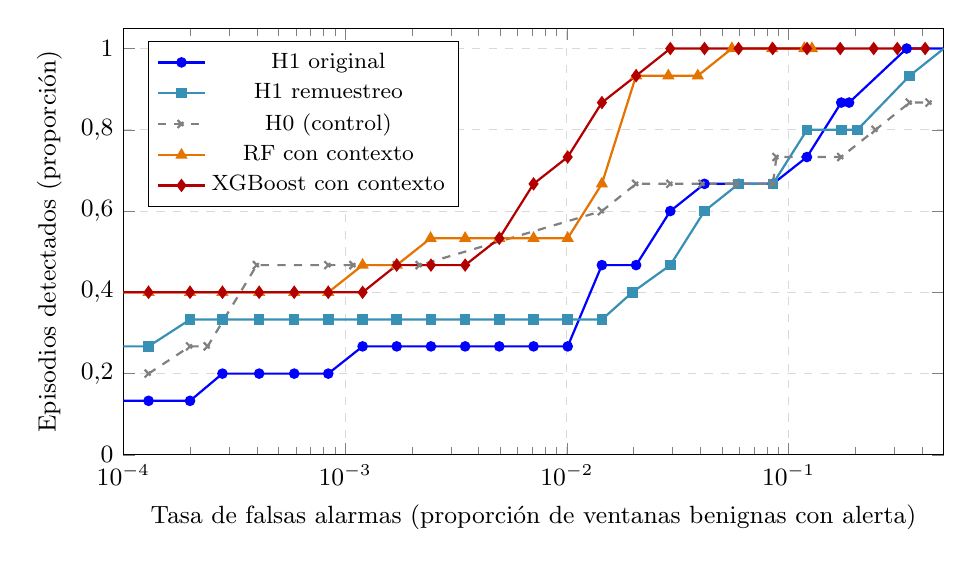
\begin{tikzpicture}
\begin{semilogxaxis}[
    width=12cm, height=7cm,
    xmin=0.0001, xmax=0.5, ymin=0, ymax=1.05,
    xlabel={Tasa de falsas alarmas (proporción de ventanas benignas con alerta)},
    ylabel={Episodios detectados (proporción)},
    grid=major, grid style={dashed,gray!30},
    tick label style={font=\small}, label style={font=\small},
    legend pos=north west, legend style={font=\footnotesize},
    /pgf/number format/use comma,
]
\addplot[thick, blue, mark=*, mark size=1.5pt] coordinates {(0.00009,0.133) (0.00013,0.133) (0.00020,0.133) (0.00028,0.200) (0.00041,0.200) (0.00059,0.200) (0.00084,0.200) (0.00120,0.267) (0.00171,0.267) (0.00244,0.267) (0.00348,0.267) (0.00496,0.267) (0.00708,0.267) (0.01009,0.267) (0.01439,0.467) (0.02053,0.467) (0.02928,0.600) (0.04176,0.667) (0.05957,0.667) (0.08494,0.667) (0.12094,0.733) (0.17270,0.867) (0.18741,0.867) (0.34071,1.000) (0.50117,1.000)};
\addlegendentry{H1 original}
\addplot[thick, cyan!70!black, mark=square*, mark size=1.5pt] coordinates {(0.00009,0.267) (0.00013,0.267) (0.00020,0.333) (0.00028,0.333) (0.00041,0.333) (0.00059,0.333) (0.00084,0.333) (0.00120,0.333) (0.00171,0.333) (0.00244,0.333) (0.00348,0.333) (0.00496,0.333) (0.00708,0.333) (0.01009,0.333) (0.01439,0.333) (0.01974,0.400) (0.02928,0.467) (0.04176,0.600) (0.05957,0.667) (0.08494,0.667) (0.12114,0.800) (0.17278,0.800) (0.20425,0.800) (0.35142,0.933) (0.50117,1.000)};
\addlegendentry{H1 remuestreo}
\addplot[thick, gray, dashed, mark=x, mark size=2pt] coordinates {(0.00013,0.200) (0.00020,0.267) (0.00024,0.267) (0.00040,0.467) (0.00084,0.467) (0.00109,0.467) (0.00171,0.467) (0.00217,0.467) (0.01439,0.600) (0.02052,0.667) (0.02928,0.667) (0.04088,0.667) (0.05859,0.667) (0.08494,0.667) (0.08813,0.733) (0.17259,0.733) (0.24631,0.800) (0.35142,0.867) (0.43172,0.867)};
\addlegendentry{H0 (control)}
\addplot[thick, orange!90!black, mark=triangle*, mark size=1.8pt] coordinates {(0.00009,0.400) (0.00013,0.400) (0.00020,0.400) (0.00028,0.400) (0.00041,0.400) (0.00059,0.400) (0.00084,0.400) (0.00120,0.467) (0.00171,0.467) (0.00243,0.533) (0.00348,0.533) (0.00496,0.533) (0.00708,0.533) (0.01009,0.533) (0.01439,0.667) (0.02052,0.933) (0.02869,0.933) (0.03895,0.933) (0.05549,1.000) (0.08423,1.000) (0.11769,1.000) (0.12739,1.000)};
\addlegendentry{RF con contexto}
\addplot[thick, red!70!black, mark=diamond*, mark size=1.8pt] coordinates {(0.00009,0.400) (0.00013,0.400) (0.00020,0.400) (0.00028,0.400) (0.00041,0.400) (0.00059,0.400) (0.00084,0.400) (0.00120,0.400) (0.00171,0.467) (0.00244,0.467) (0.00348,0.467) (0.00496,0.533) (0.00708,0.667) (0.01009,0.733) (0.01439,0.867) (0.02053,0.933) (0.02928,1.000) (0.04175,1.000) (0.05947,1.000) (0.08474,1.000) (0.12105,1.000) (0.17087,1.000) (0.24187,1.000) (0.30911,1.000) (0.41252,1.000)};
\addlegendentry{XGBoost con contexto}
\end{semilogxaxis}
\end{tikzpicture}
\caption[Episodios detectados frente a la tasa de falsas alarmas en Unraveled.]{Episodios detectados frente a la tasa de falsas alarmas en la partición de prueba de Unraveled, al variar el umbral $\tau$. Los modelos de referencia usan atributos continuos y datos originales. Fuente: Elaboración propia.}
\label{fig:curva_ttd_fpr}
\end{figure}
\FloatBarrier

El umbral calibrado en validación no conserva la tasa de falsas alarmas objetivo en la partición de prueba. En Unraveled, el umbral calibrado para un 0,1~\% produce un 0,75~\% de falsas alarmas en el HMM supervisado y entre 0,5~\% y 1,6~\% en los modelos de referencia, y en DAPT2020 el umbral calibrado para un 1~\% produce un 1,6~\% en el HMM. Por ello, las comparaciones de este capítulo se basan en la curva y no en el punto de operación calibrado.

La tasa de detección previa a la exfiltración resultó nula en todas las configuraciones, pero este valor no refleja el desempeño de los modelos. De los seis episodios de prueba de Unraveled que contienen exfiltración, cinco comienzan directamente con ella, y en DAPT2020 ocurre lo mismo con los dos episodios que la contienen. En esos casos no existe un instante anterior a la exfiltración dentro del episodio en que se pueda emitir una alerta. Esto se debe a que, en Unraveled, cada host cumple casi siempre un único papel en la campaña, de modo que la progresión entre etapas se observa en la red completa y no dentro de la secuencia de un mismo host.

\subsection{Sensibilidad de la configuración}
\label{sec:res_sensibilidad}
Para evaluar las decisiones de preprocesamiento sin recurrir a la partición de prueba, se repitieron las configuraciones del HMM sobre Unraveled variando un aspecto a la vez y evaluando en la partición de validación. La Tabla~\ref{tab:sensibilidad} presenta los resultados de H1 con datos originales. En todas las variantes, el umbral se calibra sobre la misma partición evaluada, por lo que la tasa de falsas alarmas se mantiene en torno al 0,1~\% y las métricas de detección son comparables entre filas.

\begin{table}[h!]
\centering
\small
\renewcommand{\arraystretch}{1.25}
\begin{tabular}{|l|c|c|c|c|c|c|c|c|}
\hline
\textbf{Variante} & $\boldsymbol{M}$ & \textbf{Rec.} & \textbf{Foot.} & \textbf{Lat.} & \textbf{Exf.} & \textbf{Macro} & \textbf{Detec.} & \textbf{TTD} \\ \hline
Base ($\Delta t$ = 5 min, p50 y p95) & 82 & 0,000 & 0,937 & 0,377 & 0,911 & 0,556 & 2/7 & 30 \\ \hline
$\Delta t$ = 1 min & 82 & 0,000 & 0,882 & 0,762 & 0,942 & 0,646 & 3/7 & 9 \\ \hline
$\Delta t$ = 15 min & 82 & 0,000 & 0,639 & 0,422 & 0,372 & 0,358 & 3/7 & 60 \\ \hline
Terciles & 82 & 0,000 & 0,936 & 0,531 & 0,987 & 0,613 & 3/7 & 15 \\ \hline
Solo p95 & 17 & 0,000 & 0,727 & 0,212 & 0,093 & 0,258 & 3/7 & 895 \\ \hline
Encubrimiento excluido & 82 & 0,000 & 0,937 & 0,377 & 0,911 & 0,556 & 2/7 & 30 \\ \hline
\end{tabular}
\caption[Sensibilidad de la configuración del HMM en la partición de validación de Unraveled.]{Sensibilidad de la configuración del HMM (H1 con datos originales) en la partición de validación de Unraveled. $M$: tamaño del alfabeto. Demás columnas como en la Tabla~\ref{tab:res_unraveled}. Fuente: Elaboración propia.}
\label{tab:sensibilidad}
\end{table}
\FloatBarrier

La ventana de un minuto obtiene el mayor $F_1$-score macro, principalmente porque duplica el $F_1$-score del movimiento lateral, y reduce la mediana del tiempo hasta la detección de 30 a 9 minutos. Parte de esta reducción se explica porque una ventana más corta disminuye también la resolución mínima del tiempo hasta la detección. Su costo es computacional: genera cinco veces más ventanas, y su ejecución tomó 43 minutos frente a menos de 10 en las otras sensibilidades. La ventana de quince minutos empeora el desempeño en el \textit{foothold} y en la exfiltración.

En la discretización, los terciles superan a los cortes en los percentiles 50 y 95, con un $F_1$-score macro de 0,613. Este resultado contradice lo que se esperaba al diseñar la discretización, que con terciles casi todas las ventanas de ataque cayeran en el mismo nivel. Usar solo el corte en el percentil 95 reduce el alfabeto a 17 símbolos y degrada el desempeño en el \textit{foothold}, el movimiento lateral y la exfiltración.

La exclusión del encubrimiento produce exactamente los mismos resultados que la configuración base, porque en Unraveled el encubrimiento ocurre solo en la partición de prueba. Esta decisión no puede evaluarse en validación y se contrastará en la validación cruzada por día.

En todas las variantes, el refinamiento con Baum-Welch volvió a ser descartado por la verificación posterior, y el reconocimiento no fue identificado. En cambio, la exfiltración se identifica en validación con un $F_1$-score de 0,911 en la configuración base, mientras que en prueba no se identifica (Tabla~\ref{tab:res_unraveled}). Esta diferencia indica que el comportamiento de la exfiltración cambia entre ambos periodos. Como cada variante se evaluó por separado y la partición de validación contiene solo siete episodios, estos resultados orientan la configuración que se congelará para la evaluación definitiva, pero aún no la determinan. En particular, falta evaluar la combinación de una ventana de un minuto con la discretización por terciles.

\section{Análisis}
\label{sec:analisis_preliminar}
Respecto de las hipótesis de trabajo planteadas en el diseño experimental, los resultados preliminares no respaldan por ahora la primera: a igual tasa de falsas alarmas, el HMM no detecta las campañas antes ni con mayor frecuencia que los modelos de referencia. La segunda hipótesis sí se observa, ya que los modelos de referencia alcanzan un $F_1$-score por ventana superior al del HMM en ambos conjuntos. Los resultados sí confirman dos decisiones del diseño: la estimación supervisada mantiene la correspondencia entre estados y etapas que el entrenamiento no supervisado pierde, y la verificación posterior impide que el refinamiento con Baum-Welch degrade esa correspondencia.

Los resultados también identifican los siguientes aspectos del diseño que requieren ajuste:
\begin{enumerate}
    \item \textbf{Nivel de la secuencia.} Como cada host de Unraveled cumple casi siempre un solo papel, la estructura de transiciones del HMM tiene poca progresión que modelar dentro de una secuencia. Se evaluará combinar las probabilidades filtradas de todos los hosts en una línea de tiempo de la campaña a nivel de red, en la que la progresión entre etapas sí es observable y la detección previa a la exfiltración puede medirse.
    \item \textbf{Observables de la exfiltración.} Ningún modelo identifica la exfiltración de prueba en Unraveled con los cuatro atributos actuales, aunque el HMM sí la identifica en validación. Se analizará qué cambia en el tráfico de exfiltración entre ambos periodos y se evaluará incorporar un atributo que acumule el volumen saliente de un host a lo largo de varias ventanas.
    \item \textbf{Calibración del umbral.} La tasa de falsas alarmas en prueba supera varias veces la objetivo. Se evaluará calibrar el umbral con más días de validación y reportar las métricas de detección siempre junto con la curva completa.
    \item \textbf{Configuración del preprocesamiento.} En validación, la ventana de un minuto y la discretización por terciles superaron a la configuración base. Se evaluará su combinación antes de congelar la configuración.
    \item \textbf{Robustez de la estimación.} Con 15 episodios en Unraveled y 8 en DAPT2020, un episodio cambia la tasa de detección en 6,7 y 12,5 puntos porcentuales, respectivamente. La validación cruzada agrupada por día y el análisis separado por grupo atacante, previstos en el plan, permitirán estimar la variabilidad de estos resultados.
\end{enumerate}

Estos resultados se obtuvieron sobre la partición de prueba con fines exploratorios. Las decisiones de configuración que se tomen a partir de ellos se basarán en la partición de validación, y la evaluación definitiva en prueba se realizará una sola vez, con la configuración congelada.

\chapter{Conclusión}
El presente Informe Final de Seminario de Título consolida la fundamentación metodológica, el estado del arte, el diseño y una primera implementación de un sistema probabilístico basado en Cadenas Ocultas de Markov (HMM) para la detección temprana de Amenazas Persistentes Avanzadas (APT).

La Revisión Sistemática de la Literatura, conducida bajo las directrices de Kitchenham y documentada según la declaración PRISMA 2020, analizó un corpus de 77 estudios primarios de Scopus, Web of Science e IEEE Xplore y evidenció cuatro brechas: la dependencia de alertas previamente correlacionadas, la escasa validación de modelos HMM sobre flujos de tráfico, la limitada representatividad temporal de los conjuntos de datos y el predominio de métricas globales como \textit{Accuracy}, que enmascaran el desempeño frente a las clases minoritarias.

Para responder a estos vacíos, la propuesta adoptó la metodología Design Science Research (DSR) y formuló un HMM generativo que vincula directamente el tráfico de red con las etapas del ataque, evaluado sobre DAPT2020 y Unraveled para asegurar tanto la comparabilidad con el estado del arte como la validez ecológica sobre trazas de varias semanas.

El prototipo implementado (Capítulo~\ref{cap:experimentos}) confirma que la estimación supervisada mantiene la correspondencia entre estados y etapas que el entrenamiento no supervisado pierde, y que la verificación posterior impide que el refinamiento con Baum-Welch la degrade. A su vez, muestra que con la configuración actual los modelos de referencia superan al HMM en la clasificación por ventana y en la detección a igual tasa de falsas alarmas.

El trabajo futuro se concentrará en:
\begin{enumerate}
    \item Incorporar una línea de tiempo de la campaña a nivel de red y un atributo de volumen saliente acumulado para la exfiltración.
    \item Seleccionar y congelar en validación la configuración del preprocesamiento, incluida la combinación de la ventana de un minuto con la discretización por terciles.
    \item Contrastar las estrategias frente al desbalance que preservan la estructura temporal de las secuencias, reservando SMOTE para los modelos de referencia.
    \item Evaluar el modelo por etapa y en detección temprana frente a la tasa de falsas alarmas, con validación cruzada por día, y compararlo con Random Forest y XGBoost bajo las mismas condiciones.
\end{enumerate}

Con ello, se busca proporcionar un artefacto funcional que reduzca el tiempo de exposición frente a campañas dirigidas en infraestructuras críticas.

\chapter{Declaración sobre el uso de herramientas de Inteligencia Artificial}

En concordancia con las directrices institucionales sobre integridad académica y el uso ético de tecnologías generativas, se declara que durante el desarrollo de este trabajo se utilizaron herramientas basadas en Modelos de Lenguaje de Gran Escala (LLM), específicamente Gemini \parencite{google2024gemini} y Claude \parencite{anthropic2024claude}, actuando estrictamente como asistentes de soporte técnico y de redacción, y en ningún caso como fuentes de autoridad conceptual o primaria.

\section{Alcance y propósito del uso}
El empleo de dichas herramientas se restringió a las siguientes actividades auxiliares:
\begin{enumerate}
    \item \textbf{Asistencia en composición y formateo en LaTeX:} Apoyo en la resolución de desbordes marginales en tablas complejas, diseño de estructuras tabulares mediante paquetes especializados (\texttt{tabularx}) y verificación de la sintaxis en la tipografía de matrices y ecuaciones matemáticas.
    \item \textbf{Revisión de estilo y coherencia discursiva:} Asistencia en la identificación de redundancias textuales, corrección de puntuación y mejora de fluidez en borradores preliminares, asegurando en todo momento que la argumentación, ideas centrales y formulaciones representen la autoría de la estudiante.
    \item \textbf{Soporte conceptual en diseño algorítmico:} Consulta sobre sintaxis de dependencias en Python (\texttt{hmmlearn}, \texttt{pandas}) y validación de la lógica estructural en la presentación de algoritmos probabilísticos.
\end{enumerate}

\section{Control de veracidad y responsabilidad personal}
Se subraya que ningún contenido generado automáticamente fue admitido sin una evaluación crítica reflexiva. Toda definición conceptual, formulación estadística, algoritmo matemático y elemento de la revisión sistemática de la literatura fue verificado directamente a partir de las fuentes bibliográficas primarias indexadas. La autoría, análisis crítico, interpretación de evidencias y decisiones metodológicas adoptadas en este informe son de exclusiva responsabilidad de la autora.

\printbibliography[title={Referencias}]

% ANEXOS
\appendix
\renewcommand{\appendixname}{Anexo}
\chapter{Modelo probabilístico implementado en Python}
\label{anx:modelo}
Este anexo reproduce el módulo \texttt{hmm.py} del prototipo descrito en el Capítulo~\ref{cap:experimentos}, que implementa el modelo $\lambda = (A, B, \pi)$ definido en la Sección~\ref{sec:modelo_formal} y la estrategia de correspondencia entre estados y etapas de la Sección~\ref{sec:correspondencia}. La Tabla~\ref{tab:anexo_funciones} relaciona cada función del módulo con el elemento de la propuesta que implementa.

\begin{table}[h!]
\centering
\small
\renewcommand{\arraystretch}{1.25}
\begin{tabularx}{\textwidth}{|>{\raggedright\arraybackslash}p{4.6cm}|>{\raggedright\arraybackslash}X|}
\hline
\textbf{Función} & \textbf{Elemento de la propuesta} \\ \hline
\texttt{mascara\_estructural} & Ceros estructurales de la matriz de transición: se prohíben las transiciones entre dos estados de ataque que no aparecen en entrenamiento \\ \hline
\texttt{HMM.supervisado} & Anclaje por supervisión: estimación de $A$, $B$ y $\pi$ por conteo de frecuencias con suavizado aditivo \\ \hline
\texttt{HMM.filtrar} & Inferencia en línea: probabilidad filtrada $P(q_t \mid O_1, \dots, O_t, \lambda)$ mediante el algoritmo \textit{forward} escalado \\ \hline
\texttt{HMM.viterbi} & Reconstrucción retrospectiva de la secuencia de estados $Q^*$ \\ \hline
\texttt{refinar\_em} & Refinamiento con Baum-Welch restringido, inicializado con la estimación supervisada y detenido según la verosimilitud en validación \\ \hline
\texttt{no\_supervisado} & Control H0: Baum-Welch sin supervisión desde diez inicializaciones aleatorias \\ \hline
\texttt{asignacion\_hungara} y \texttt{permutar} & Emparejamiento de los estados del control con las etapas mediante el algoritmo húngaro \\ \hline
\end{tabularx}
\caption{Funciones del módulo \texttt{hmm.py} y elementos de la propuesta que implementan. Fuente: Elaboración propia.}
\label{tab:anexo_funciones}
\end{table}
\FloatBarrier

El módulo utiliza constantes definidas en el módulo de configuración del prototipo: los cinco estados del modelo, con el estado benigno en la posición 0, y los suavizados de la matriz de transición y de la distribución inicial, ambos iguales a 1. Los comentarios D9 y D10 remiten a las decisiones de diseño registradas en el plan de experimentación del repositorio del proyecto, que corresponden a los ceros estructurales y al refinamiento restringido con el control no supervisado, respectivamente. Los demás módulos del prototipo, encargados de la carga de datos, la construcción de ventanas, la discretización, los modelos de referencia y las métricas, se encuentran en el mismo repositorio.

\lstinputlisting[caption={Módulo \texttt{hmm.py} del prototipo.}, label={lst:hmm}]{../src/apthmm/hmm.py}

\end{document}
